%$Header: svn://localhost/dtapublic/pubs/books/ucbka/trunk/c_cil0/c_cil0.tex 277 2019-08-13 02:35:39Z dashley $

\chapter[\ccilzeroshorttitle{}]{\ccilzerolongtitle{}}

\label{ccil0}

\beginchapterquote{``If our ancestors had invented arithmetic by counting with
                     their two fists or their eight fingers, instead of their
                     ten `digits', we would never have to worry about
                     writing binary-decimal conversion routines.
                     (And we would perhaps never have learned as much about
                     number systems.)''}
                     {Donald E. Knuth, \cite[p. 319]{bibref:b:knuthclassic2ndedvol2}}

%%%%%%%%%%%%%%%%%%%%%%%%%%%%%%%%%%%%%%%%%%%%%%%%%%%%%%%%%%%%%%%%%%%%%%%%%%
%%%%%%%%%%%%%%%%%%%%%%%%%%%%%%%%%%%%%%%%%%%%%%%%%%%%%%%%%%%%%%%%%%%%%%%%%%
%%%%%%%%%%%%%%%%%%%%%%%%%%%%%%%%%%%%%%%%%%%%%%%%%%%%%%%%%%%%%%%%%%%%%%%%%%
\section{Introduction}
%Section tag: INT0
\label{ccil0:sint0}

Low-cost microcontrollers have no support for floating-point arithmetic,
and so integer arithmetic and fixed-point arithmetic are used nearly exclusively
in embedded systems.  The ability to implement integer arithmetic
economically is a critical skill in the development of embedded
systems.

Integer arithmetic algorithms are critically important in embedded
systems for the following reasons:

\begin{itemize}
\item Mistakes in the implementation of arithmetic are frequently
      responsible for product problems.  (Mistakes are not confined
      to obvious errors---errors such as filters which do not converge
      on their input are also responsible for product problems.)
\item Floating-point arithmetic is not available or ill-advised
      for nearly all small embedded systems for the following reasons:
      \begin{itemize}
      \item Low-cost microcontrollers do not possess hardware support for
            floating-point arithmetic.
      \item Implementation of floating-point arithmetic in software is
            computationally expensive.
      \item Implementation of floating-point arithmetic in software may
            require large floating-point libraries, typically consuming
            1K-4K of ROM.
      \item Safety-critical software standards typically prohibit the
            use of floating-point arithmetic.
      \end{itemize}
\item Integer arithmetic algorithms (other than addition and subtraction)
      are quite tedious and error-prone for a software developer to design, implement, and
      unit test.  The implementation of such algorithms represents
      cost and risk.  Cost and risk benefits are achieved if the algorithms in detail are 
      available in advance (thus precluding design activities), or
      better yet if ready-to-use integer algorithm libraries are available.
\end{itemize}

This chapter describes the more fundamental principles and algorithms
(representation, fixed-point arithmetic, treatment of overflow, comparison,
addition, subtraction, multiplication, and division).  A section 
(Section \ref{ccil0:smim0}) is also included 
on miscellaneous mappings involving integers which
are not numerical in intent.
Chapter %\cdtazeroxrefhyphen\cdtazerovolarabic{} 
TBD
describes more complicated 
integer algorithms and techniques (discrete-time operations
such as filtering, integration, and differentiation as well as more
complex functions such as square root).  The split between these two chapters
is arbitrary; and in fact the material could have been divided differently
or combined.

Treatment of the topics in this chapter is largely in accordance with
Knuth \cite{bibref:b:knuthclassic2ndedvol2}.  The principal issues in 
the implementation of integer algorithms are:

\begin{itemize}
\item \textbf{How to use the arithmetic [or other] instructions provided by the machine to
      operate on larger operands.}  Microcontrollers typically provide arithmetic
      instructions (comparison, shifting, addition, subtraction, and often but not
      always multiplication and/or division) that operate on 8-bit or 16-bit integers.  
      A key question
      is how small-operand instructions ``scale up''---that is, if and how they can
      be used to assist in the implementation of integer arithmetic for much larger 
      operands.
\item \textbf{The order of the algorithm involved.}  The order of algorithms
      is a complicated issue when applied to microcontroller work.  Many sophisticated
      algorithms have a breakpoint below which they are less economical than
      an inferior algorithm.  Some applications (such as generating cryptographic keys
      when integers thousands of bits long must be tested for primality) will
      benefit from sophisticated algorithms becuase the operand sizes are large enough
      to pass any such breakpoints.  However, in microcontroller work, the need to manipulate
      integers longer than 64 bits is very rare; thus, the breakpoints that indicate the
      use of more sophisticated algorithms may not be reached.  In microcontroller work,
      depending on the operand sizes, there are circumstances in which an
      $O(n^2)$ algorithm may be preferable to an $O(\log n)$ algorithm.  Generally,
      the order of algorithms must be balanced against operand sizes.
\end{itemize}

We do diverge from Knuth in some areas.  The most prominent divergence is
in the proofs offered for some important theorems and lemmas.  Knuth 
employs contrapositive proof formats in many circumstances, whereas we prefer
to use linear proofs that are more understandable to engineers and microcontroller
software developers.

%%%%%%%%%%%%%%%%%%%%%%%%%%%%%%%%%%%%%%%%%%%%%%%%%%%%%%%%%%%%%%%%%%%%%%%%%%
%%%%%%%%%%%%%%%%%%%%%%%%%%%%%%%%%%%%%%%%%%%%%%%%%%%%%%%%%%%%%%%%%%%%%%%%%%
%%%%%%%%%%%%%%%%%%%%%%%%%%%%%%%%%%%%%%%%%%%%%%%%%%%%%%%%%%%%%%%%%%%%%%%%%%
\section[Paradigms And Principles]
        {Paradigms And Principles Of Microcontroller Arithmetic}
%Section tag: PPM0
\label{ccil0:sppm0}

How should one think about microcontroller arithmetic?  What principles
guide us in its design and implementation?  In this section,
we provide some general principles and paradigms of thought.


%%%%%%%%%%%%%%%%%%%%%%%%%%%%%%%%%%%%%%%%%%%%%%%%%%%%%%%%%%%%%%%%%%%%%%%%%%
%%%%%%%%%%%%%%%%%%%%%%%%%%%%%%%%%%%%%%%%%%%%%%%%%%%%%%%%%%%%%%%%%%%%%%%%%%
%%%%%%%%%%%%%%%%%%%%%%%%%%%%%%%%%%%%%%%%%%%%%%%%%%%%%%%%%%%%%%%%%%%%%%%%%%
\subsection{Microcontroller Arithmetic As An Accident Of Silicon Design}
%Subsection tag: MAS0
\label{ccil0:sppm0:smas0}

In chapters
\cfryzeroxrefhyphen{}\ref{cfry0},
\ccfrzeroxrefhyphen{}\ref{ccfr0},
and 
\cratzeroxrefhyphen{}\ref{crat0} 
we consider rational approximation,
both in the form $h/k$ and $h/2^q$.  Both forms of rational approximation
tend to be effective because we know that all modern processors possess
shift instructions, most possess integer multiply instructions, and many 
possess integer divide instructions.  In other words, the design
of the machine instruction set drives the strategies for implementation
of arithmetic, and makes some strategies attractive.

Similarly, the observation that all microcontrollers provide instructions
for integer arithmetic creates the attractiveness of fixed-point arithmetic.

Thus, we might view our approaches to microcontroller arithmetic as 
an ``accident'' of silicon design, or as being driven by silicon
design.

Generally, we seek to determine the best way to use the primitive
operations provided by the machine (the instruction set) to 
accomplish the mappings of interest.

The ``classic'' algorithms 
presented by Knuth 
Knuth (\cite[pp. 265-284]{bibref:b:knuthclassic2ndedvol2}) are especially
designed to use the ``small'' addition, subtraction, multiplication, and
division provided by the machine to add, subtract, multiply, and divide arbitrarily
large integers.  In 
\cite[pp. 265-266]{bibref:b:knuthclassic2ndedvol2}) Knuth writes:

\begin{quote}
\emph{The most important fact to understand about extended-precision numbers
is that they may be regarded as numbers written in radix-$w$ notation,
where $w$ is the computer's word size.  For example, an integer that
fills 10 words on a computer whose word size is $w=10^{10}$ has 100
decimal digits; but we will consider it to be a 10-place number to
the base $10^{10}$.  This viewpoint is justified for the same reason
that we may convert, say, from binary to hexadecimal notation,
simply by grouping the bits together.}

\emph{In these terms, we are given the following primitive operations to work with:}

\begin{itemize}
\item \emph{a$_0$) addition or subtraction of one-place integers, giving a one-place
             answer and a carry;}
\item \emph{b$_0$) multiplication of a one-place integer by another one-place integer,
             giving a two place answer;}
\item \emph{c$_0$) division of a two-place integer by a one-place integer, 
             provided that the quotient is a one-place integer, and yielding
			    also a one-place remainder.}
\end{itemize}

\noindent{}\emph{By adjusting the word size, if necessary, nearly all computers
will have these three operations available; so we will construct algorithms
(a), (b), and (c) mentioned above in terms of the primitive operations
(a$_0$), (b$_0$), and (c$_0$).}

\emph{Since we are visualizing extended-precision integers as base $b$ numbers, it is
sometimes helpful to think of the situation when $b = 10$, and to imagine
that we are doing the arithmetic by hand.  Then operation (a$_0$) is analogous
to memorizing the addition table; (b$_0$) is analogous to memorizing the 
multiplication table, and (c$_0$) is essentially memorizing the multiplication
table in reverse.  The more complicated operations (a), (b), (c) on
high-precision numbers can now be done using simple addition, subraction,
multiplication, and long-division procedures that children are taught
in elementary school.}
\end{quote}

The critical issue for implementation of integer arithmetic with large operands
is how to use small-operand instructions to operate on larger operands---in other words,
how to ``scale up'' the capability provided by the instruction set. 


%%%%%%%%%%%%%%%%%%%%%%%%%%%%%%%%%%%%%%%%%%%%%%%%%%%%%%%%%%%%%%%%%%%%%%%%%%
%%%%%%%%%%%%%%%%%%%%%%%%%%%%%%%%%%%%%%%%%%%%%%%%%%%%%%%%%%%%%%%%%%%%%%%%%%
%%%%%%%%%%%%%%%%%%%%%%%%%%%%%%%%%%%%%%%%%%%%%%%%%%%%%%%%%%%%%%%%%%%%%%%%%%
\subsection{Microcontroller Arithmetic As A Mapping From Quantized Domain To
            Quantized Range}
%Subsection tag: MAM0
\label{ccil0:sppm0:smam0}

Microcontroller software accepts inputs which are quantized.  In nearly all cases,
this involves a mapping from $\vworkrealset$ to $\vworkintset$.  Often, because
microcontroller products are optimized for cost, the quantization hardware
delivers quite poor precision, frequently less than 8 bits.  

When a quantized input is accepted, it defines an inquality.  Knowledge of
the quantized input (an integer) confines the actual input (a real
number, before 
quantization) to an interval.  With a low-cost hardware design, the
interval can be fairly large.  Usually, by adding cost, the
interval can be made smaller.

Microcontroller outputs tend to be quantized as well, so it is
accurate to also characterize outputs as integers.  For example, a PWM signal
generated by a microcontroller or the output of a D/A converter is
controlled by data that is an integer.  Like inputs, often the ``granularity''
with which outputs can be controlled is quite coarse---again, 8 bits or
less is not uncommon.

Thus, we may view microcontroller software as a mapping from poor-quality
inputs to poor-quality outputs.

In such a framework, where the nature of inputs and outputs introduces
substantial error, it is imperative not to introduce additional error
in computer arithmetic.  In other words, given inputs which are 
integers, the responsibility of the software is to choose the best 
integers as outputs.  Usually this means that calculations should be
devised so as not to lose any information (i.e.
not to lose remainders, for example).  Losing information is usually
equivalent to not being able to make the most correct mapping from input
to output.  ``Lossy'' arithmetic can degrade the performance of a system,
since poor arithmetic may compound an inexpensive hardware design.


%%%%%%%%%%%%%%%%%%%%%%%%%%%%%%%%%%%%%%%%%%%%%%%%%%%%%%%%%%%%%%%%%%%%%%%%%%
%%%%%%%%%%%%%%%%%%%%%%%%%%%%%%%%%%%%%%%%%%%%%%%%%%%%%%%%%%%%%%%%%%%%%%%%%%
%%%%%%%%%%%%%%%%%%%%%%%%%%%%%%%%%%%%%%%%%%%%%%%%%%%%%%%%%%%%%%%%%%%%%%%%%%
\subsection{Microcontroller Arithmetic As A Simulation Of Continuous Controllers}
%Subsection tag: MAE0
\label{ccil0:sppm0:smae0}

Control systems have not always employed digital controllers.
Many books and web sites (see \cite{bibref:w:historycontrol01}, for example)
discuss the historical development of feedback control.  Controllers
have not historically been digital, or even electronic.
Early controllers for governing steam devices or windmills were
ultimately mechanical, and relied upon inertia or other physical
properties.  It is possible to realize abstract notions
(integrators, differentiators, gains) using hydraulic systems or other mechanical systems;
and in fact hydraulic feedback controllers were used in early rockets
and aircraft.  Very naturally, abstract notions (integrators,
differentiators, gains) can be implemented using analog
electronic components.  The most common implementations involve
operational amplifiers, and the behavior of such implementations comes
very close to the ideal mathematical models.

Mechanical, hydraulic, and non-digital electronic controllers have
one very desirable characteristic---\emph{clipping}.  If, for example,
one provides an analog differentiator with a $dV/dt$ which
is too large, the output that the differentiator can 
provide is limited, usually by the supply voltage available to an operational
amplifier.
The differentiator \emph{must} clip.

Clipping often leads to behavior which is close to what
intuition would expect (i.e. we would present 
clipping as an occasional advantage).  For example, if an input to
an analog control system suffers a failure, the behavior
the of the controller is limited, as is its internal
state.  Similarly, when the
input is restored, the controller will usually recover 
in a reasonable time because the
state of the controller (typically maintained in capacitors) is limited
in the magnitude it can attain.

We might view a digital controller as an emulation of
an analog controller.  We may want to cause the
controller to have limits (i.e. rails) internally, for
example to prevent excessive integrator ``windup''.  We discuss
this further in Section \ref{ccil0:sode0}.


%%%%%%%%%%%%%%%%%%%%%%%%%%%%%%%%%%%%%%%%%%%%%%%%%%%%%%%%%%%%%%%%%%%%%%%%%%
%%%%%%%%%%%%%%%%%%%%%%%%%%%%%%%%%%%%%%%%%%%%%%%%%%%%%%%%%%%%%%%%%%%%%%%%%%
%%%%%%%%%%%%%%%%%%%%%%%%%%%%%%%%%%%%%%%%%%%%%%%%%%%%%%%%%%%%%%%%%%%%%%%%%%
\section{Practical Design Issues}
%Section tag: PDI0
\label{ccil0:spdi0}

In this section, we consider practical issues surrounding the design
and construction of a set of integer arithmetic subroutines.
In practice, such a collection of subroutines is likely to be
arranged into a library.  The purpose of the library would be to
free the clients (or callers) of the library from the complexity of 
large integer calculations.

The design decisions surrounding the construction of a library vary in
the objectivity with which they can be approached.  Some design decisions
(such as the best mechanism for passing parameters) can be approached
rigorously because the measures of goodness are unequivocal (minimal ROM consumption
or execution time, for example).  However, other design decisions, particulary the
decision of the exact nature of the interface between an arithmetic library and
its clients, are more subjective.  One size does \emph{not} fit all.


%%%%%%%%%%%%%%%%%%%%%%%%%%%%%%%%%%%%%%%%%%%%%%%%%%%%%%%%%%%%%%%%%%%%%%%%%%
%%%%%%%%%%%%%%%%%%%%%%%%%%%%%%%%%%%%%%%%%%%%%%%%%%%%%%%%%%%%%%%%%%%%%%%%%%
%%%%%%%%%%%%%%%%%%%%%%%%%%%%%%%%%%%%%%%%%%%%%%%%%%%%%%%%%%%%%%%%%%%%%%%%%%
\subsection{Parameter Passing And Temporary Storage Mechanisms}
%Subsection tag: PPM0
\label{ccil0:spdi0:sppm0}

In small microcontroller work, the desire to save ROM and execution time
may lead to inelegant software construction.  Because an arithmetic library
used in microcontroller work may be called from many different places 
throughout ROM, serious thought should be given to optimizing the 
parameter passing mechanisms, even perhaps at the expense of elegance.
The way in which the arithmetic library allocates temporary storage is
also a point of concern, because the most elegant way of allocating temporary
storage (on the stack) may either not be feasible (because of the possibility
of stack overflow) or may not be efficient (because the addressing modes of
the machine make data on the stack inefficient to address).  In this section
we discuss both parameter passing and temporary storage mechanisms.

In the remainder of the discussion, we make the following assumptions
about software architecture.

\begin{enumerate}
\item \textbf{The arithmetic library need not be re-entrant.}
      Most ``small'' microcontroller software loads use a non-preemptive
      scheduling paradigm, so this is a reasonable assumption.  We also
      make the reasonable assumption that ISR's may not make calls into 
      the arithmetic library.
\item \textbf{Dynamic memory allocation, other than on the stack,
      is not allowed by the software architecture.}  This is also
      a reasonable assumption in ``small'' microcontroller software.
\end{enumerate}

%%%%%%%%%%%%%%%%%%%%%%%%%%%%%%%%%%%%%%%%%%%%%%%%%%%%%%%%%%%%%%%%%%%%%%%%%%
%%%%%%%%%%%%%%%%%%%%%%%%%%%%%%%%%%%%%%%%%%%%%%%%%%%%%%%%%%%%%%%%%%%%%%%%%%
%%%%%%%%%%%%%%%%%%%%%%%%%%%%%%%%%%%%%%%%%%%%%%%%%%%%%%%%%%%%%%%%%%%%%%%%%%
\subsubsection{Parameter Passing Mechanisms}
%Subsubsection tag: PPM0
\label{ccil0:spdi0:sppm0:sppm0}

If an arithmetic library exists in a microcontroller software load,
it may be called many times throughout ROM.  Thus, the parameter 
passing mechanisms chosen may have a large effect on ROM consumption
(due to the setup required for each subroutine call multiplied by
many instances throughout ROM) and execution time
(because in microcontroller software longer instructions nearly always
require more time).  Because of the criticality of ROM consumption,
parameter passing mechanisms that lack elegance may be attractive.

In the category of parameter passing, we also include the way in which
return value(s) are passed back to the caller.

The following parameter-passing mechanisms may be employed:

\begin{enumerate}
\item \textbf{Pass by value as storage class \emph{automatic}.}
      The most common scenario is that the arithmetic
      library is written in assembly-language to be called from
      `C', and so the assembly-language subroutines must adhere to the
      parameter-passing conventions used by the compiler.
      This usually means that the entire input or output value
      will be passed in CPU registers or on the stack.  Somewhat rarely, 
      a compiler will pass parameters in static locations.\footnote{The
      usual reason for a `C' compiler to pass parameters in static locations
      is because the instruction set of the machine was not designed for
      higher-level languages, and references to [usually \emph{near}] memory
      are cheaper than stack references.  Such compilers also typically 
      analyze the calling tree of the program where possible and use this
      information to overlay the parameter-passing memory areas of 
      subroutines that cannot be active simultaneously.  Without the ability
      to analyze the calling tree and make overlay decisions based on it,
      memory would be exhausted, because each subroutine would need to have its
      own static storage for parameters and local variables.}
\item \textbf{Pass by reference.}
      Typically, it is convenient to pass pointer(s) to area(s) of memory
      containing input operands, and also a pointer to an area of memory
      owned by the caller which is written with the result by the arithmetic subroutine.
      The efficiency of this approach depends on the compiler and the instruction
      set of the machine.  If the instruction set of the machine cannot 
      make effective use of pointers or stack frames, an arithmetic subroutine
      might be constructed so that it first copies the operands to a static area of memory
      reserved for the arithmetic library, then performs the necessary arithmetic
      operations on the operands in the static area, 
      then copies the result(s) back to the area owned by the caller.
\item \textbf{Pass by common data block.}
      In some cases, it may be preferable to reserve a block of memory in which to
      pass parameters to arithmetic library functions, and from which to retrieve
      results after an arithmetic library function returns.  The allocation of such
      a static memory block may be done manually\footnote{Note to self:  need to
      include gentleman's agreements on memory usage in my note on software architecture.}
      or automatically (by development tools which can analyze the function calling tree and
      manage the overlaying).
\end{enumerate}



%%%%%%%%%%%%%%%%%%%%%%%%%%%%%%%%%%%%%%%%%%%%%%%%%%%%%%%%%%%%%%%%%%%%%%%%%%
%%%%%%%%%%%%%%%%%%%%%%%%%%%%%%%%%%%%%%%%%%%%%%%%%%%%%%%%%%%%%%%%%%%%%%%%%%
%%%%%%%%%%%%%%%%%%%%%%%%%%%%%%%%%%%%%%%%%%%%%%%%%%%%%%%%%%%%%%%%%%%%%%%%%%
\subsubsection{Temporary Storage Mechanisms}
%Subsubsection tag: TSM0
\label{ccil0:spdi0:sppm0:stsm0}

Need to indicate clearly on section on software architectures the
primary temporary storage mechanisms:

\begin{itemize}
\item Stack.
\item Memory block with overlay functionality.
\end{itemize}

Need to expand software architecture section to cover this, so don't
discuss here.


%%%%%%%%%%%%%%%%%%%%%%%%%%%%%%%%%%%%%%%%%%%%%%%%%%%%%%%%%%%%%%%%%%%%%%%%%%
%%%%%%%%%%%%%%%%%%%%%%%%%%%%%%%%%%%%%%%%%%%%%%%%%%%%%%%%%%%%%%%%%%%%%%%%%%
%%%%%%%%%%%%%%%%%%%%%%%%%%%%%%%%%%%%%%%%%%%%%%%%%%%%%%%%%%%%%%%%%%%%%%%%%%
\subsection{Reporting Of Overflow, Underflow, And Domain Errors}
%Subsection tag: OUD0
\label{ccil0:spdi0:soud0}

Long integer data types used in microcontroller work are typically
of a static size (they cannot grow in size in as operations are 
performed on them).  The reason for the typical static sizes is that
dynamic allocation (except for allocation and
deallocation on the stack as subroutines
are called and return) is rarely used in small microcontroller work.
It will come about in the normal usage of an integer arithmetic 
library that an attempt will be made to operate on integers in
a way which generates an overflow, generates an
underflow, or
represents a domain error (division by zero or
square root of a negative integer, for example).
An important design decision is how such normal exceptions should be
handled.

Possible design decisions in this area are:

\begin{enumerate}
\item \label{enum:ccil0:spdi0:soud0:01:01}
      \textbf{To design arithmetic subroutines so that exceptions are not
      possible.}  
      For example, multiplying an $m$-word integer by an $n$-word integer
      will always generate an integer that will fit within $m+n$ words.
      If a multiplication subroutine is designed so that the caller must
      provide an $m$-word operand and an $n$-word operand and a pointer to
      an $(m+n)$-word area of memory for the result, an overflow cannot occur.
      Such a design decision essentially pushes overflow detection back up to
      the callers of arithmetic subroutines.
\item \label{enum:ccil0:spdi0:soud0:01:02}
      \textbf{To design arithmetic subroutines so that exceptions are possible,
      but not to detect the exceptions, thus providing an implementation that
      will produce incorrect results with some operand data values.}
      For example, if an arithmetic subroutine is designed to add an $m$-word
      operand to another $m$-word operand to produce an $m$-word result, overflow
      is possible.  A design decision to fail to detect such exceptions pushes
      the responsibility up to the callers of the arithmetic subroutines.
      Callers must devise a method for not calling arithmetic subroutines
      with data values that will cause an exception, or else to detect an exception
      when it has occurred.
\item \label{enum:ccil0:spdi0:soud0:01:03}
      \textbf{To ``rail'' the result in response to an exception.}  
      It was stated earlier that analog control system functional blocks
      built with operational 
      amplifiers typically have an output which cannot go beyond the 
      supply rails.  One may implement similar behavior in arithmetic subroutines.
      In an addition subroutine which adds two $m$-word operands to produce an
      $m$-word result (with each word having $w$ bits), it would be natural to 
      return $2^{mw}-1$ in the event of an overflow in a positive direction and 
      $-2^{mw}$ in the event of an overlfow in a negative direction.  Note that
      the caller will not be able to distinguish a ``rail'' value which represents
      a valid result from a ``rail'' value substituted to indicate an exception.
\item \label{enum:ccil0:spdi0:soud0:01:04}
      \textbf{To reserve special result data values to indicate exceptions.}
      Depending on the arithmetic subroutine being implemented, it may be possible
      to reserve certain result data values to indicate exceptions.  This approach
      is often awkward, as most mathematical subroutines are naturally defined so that
      all bit patterns in the memory reserved for the result are valid numbers.
      Additionally, with long result data values, it may not be economical to
      compare the result against the reserved exception values.  Thus, this is seldom
      an optimal way to deal with exceptions.

      Additionally, if this approach is employed, the semantics of how exception
      values combine with other exception values and data values must be decided.
\item \label{enum:ccil0:spdi0:soud0:01:05}
      \textbf{To return exception codes to the caller separate from the result data.}
      In the `C' language, pointers are often used to supply an arithmetic subroutine
      with the input operands and to provide the arithmetic subroutine with a location
      (which belongs to the caller) in which to store the result data.  Thus, the return
      value of the arithmetic subroutine (normally assigned through the subroutine name)
      is often available to return exception codes.  For example,
      a `C' function may be defined as 

      \begin{verbatim}
      unsigned char int128_add(INT128 *result, 
                               INT128 *arg1, 
                               INT128 *arg2),
      \end{verbatim}

      leaving the returned \texttt{unsigned char} value available to return
      exception information.  Note that this arrangement has the following advantages:

      \begin{enumerate}
      \item All bit patterns in the result data memory area area available
            as data bit patterns.
      \item The exception data is very economical to test, because it is placed
            in a machine-native data type.
      \item The exception data can easily be discarded or by the caller if desired.
      \item All decisions about how to handle exceptions are left to the caller. 
      \end{enumerate}
\item \label{enum:ccil0:spdi0:soud0:01:06}
      \textbf{To maintain exception data with each result integer.}
      It is possible to reserve bits for exception information which are part of the
      long integer data type.  This exception state essentially conveys 
      \emph{NaN}\footnote{\emph{N}ot \emph{a} \emph{n}umber.} information---integers with
      exception information set are not true numbers, but rather they are different from the
      true result in some way.  As with (\ref{enum:ccil0:spdi0:soud0:01:04}), the 
      semantics of how to combine NaN values and NaN values with ordinary non-NaN numbers
      must be defined.
\item \label{enum:ccil0:spdi0:soud0:01:07}
      \textbf{To maintain a global exception state variable.}
      A variable or set of variables can be reserved which hold the
      exception information, if any, from the most recent call to 
      a function in the arithmetic library.
      
      To save CPU cycles, the arithmetic library can 
      be designed so that it will assign the global exception state variable only if an 
      exception occurs---the caller then has the responsibility of clearing the exception
      state variable before making any call into the arithmetic library where the 
      exception result is of interest.  The interface between the caller and the library
      can be further optimized if the library only OR's data into the variable containing
      the exception state.  Using this optimization, the caller can clear the exception state 
      variable, make several calls into the arithmetic library, and then retrieve a meaningful
      exception state variable value summarizing several arithmetic operations.
\item \label{enum:ccil0:spdi0:soud0:01:08}
      \textbf{Hybrid approaches.}
      The approaches (\ref{enum:ccil0:spdi0:soud0:01:01})
      through (\ref{enum:ccil0:spdi0:soud0:01:07}) can be combined.
      For example, approach (\ref{enum:ccil0:spdi0:soud0:01:03})
      might be combined with approach (\ref{enum:ccil0:spdi0:soud0:01:05})
      so that exceptions are ``railed'', but the caller may also be made
      aware that an exception has occured.  Many hybrid approaches are possible.
\end{enumerate}


%%%%%%%%%%%%%%%%%%%%%%%%%%%%%%%%%%%%%%%%%%%%%%%%%%%%%%%%%%%%%%%%%%%%%%%%%%
%%%%%%%%%%%%%%%%%%%%%%%%%%%%%%%%%%%%%%%%%%%%%%%%%%%%%%%%%%%%%%%%%%%%%%%%%%
%%%%%%%%%%%%%%%%%%%%%%%%%%%%%%%%%%%%%%%%%%%%%%%%%%%%%%%%%%%%%%%%%%%%%%%%%%
\subsection{Semantics Of Combining Overflow, Underflow, And Domain Errors}
%Subsection tag: CMB0
\label{ccil0:spdi0:scmb0}

For control system arithmetic, some form of clipping as suggested
in Section \ref{ccil0:sppm0:smae0} is probably the 
best approach.  Definitely, an overflow should generate a result
which is the largest representable integer, and an
underflow should generate a result which is the smallest
representable integer.

In addition to treating an overflow by clipping, it may be 
advantageous to reserve a flag in the representation of a
multiple-precision integer to record that an overflow has occured and been clipped.
Some functions which accept the integer as input may be interested
in the value of such a flag, where othere---perhaps most---may
not.

The correct course of action in the event of a domain error (such
as division by zero) is less clear.  It is noteworthy that in a
normal control system, domain errors cannot occur (but overflows
can).

The best approach when a domain error is involved probably 
depends on the basis for the underlying calculation.  For
example, if integer division is used as part of a 
strategy for software ratiometric conversion, a value
of zero in the denominator probably represents extreme electrical
noise, and the most sane approach may be to replace the
denominator by one.  However, in other contexts it may be appropriate
to think in terms of 

\begin{equation}
\lim_{k \rightarrow 0^+} \frac{kn}{kd}
\end{equation}

\noindent{}or

\begin{equation}
\lim_{k \rightarrow 0^-} \frac{kn}{kd} .
\end{equation}

Put in other terms, there is not a clear ``one solution
meets all needs'' approach to dealing with domain
errors.

As in the case of overflows, it may be advantageous to reserve a bit
flag to signal that a domain error has occured and that the result
is not valid or not reliable.  Note that floating point chips
(such as the 80x87) provide similar indications of domain errors.

It may also be advantageous to adopt conventions for how 
overflow or domain error flags propagate through binary or
unary operators.  For example, if two numbers are multiplied, and
one of the two has the overflow flag set, it may be wise set the
overflow flag in the  result.  A scheme for how warning
flags propagate may be beneficial.


%%%%%%%%%%%%%%%%%%%%%%%%%%%%%%%%%%%%%%%%%%%%%%%%%%%%%%%%%%%%%%%%%%%%%%%%%%
%%%%%%%%%%%%%%%%%%%%%%%%%%%%%%%%%%%%%%%%%%%%%%%%%%%%%%%%%%%%%%%%%%%%%%%%%%
%%%%%%%%%%%%%%%%%%%%%%%%%%%%%%%%%%%%%%%%%%%%%%%%%%%%%%%%%%%%%%%%%%%%%%%%%%
\subsection{Variable Versus Constant Subroutine Execution Time}
%Subsection tag: VVC0
\label{ccil0:spdi0:svvc0}

As a design goal of an embedded system, we seek to minimize the
timing variability of software components.  An arithmetic subroutine
that with a high probability takes a short time to execute and with a
low probability takes a long time to execute, and where the execution
time is data dependent, is a serious risk.  An embedded software product 
may pass all release testing, but then fail in the field because of 
specific data values used in calculations.

A very conservative design goal would be to design every arithmetic subroutine
to require exactly the same execution time, regardless of data values.
This goal is not practical because machine instructions themselves
usually have a variable execution time, particularly for multiplication
and division instructions.  A fallback goal would be to avoid
large differences between minimum and maximum execution time, without
increasing the maximum execution time.  A very practical step to take
(using division as an example) 
is to insert artifical delays into easily detectable exception cases (such as
division by zero) so that the exception case takes as long as the 
minimum time for a division with valid operands.


%%%%%%%%%%%%%%%%%%%%%%%%%%%%%%%%%%%%%%%%%%%%%%%%%%%%%%%%%%%%%%%%%%%%%%%%%%
%%%%%%%%%%%%%%%%%%%%%%%%%%%%%%%%%%%%%%%%%%%%%%%%%%%%%%%%%%%%%%%%%%%%%%%%%%
%%%%%%%%%%%%%%%%%%%%%%%%%%%%%%%%%%%%%%%%%%%%%%%%%%%%%%%%%%%%%%%%%%%%%%%%%%
\section{Fixed-Point Arithmetic}
%Section tag: FPA0
\label{ccil0:sfpa0}

\emph{Fixed-point arithmetic}\index{fixed-point arithmetic} 
is a scheme for the representation
of engineering quantities (conceptually real numbers with optional
units) by integers so that calculations can be performed
on these quantitites using [usually multiple-precision]
integer arithmetic.

In discussing fixed-point arithmetic,
we must be careful to distinguish between the 
\emph{represented value} (the engineering quantity)
and the \emph{representation} (the integer which represents 
the engineering quantity).  In most cases, we must also
be careful to devise a system to track the units of the 
represented values, as, especially with control systems,
the units of represented values (due to integration and 
differentiation) can become very complex
and mistakes are easy to make.

Fixed-point arithmetic is the dominant paradigm of construction
for calculations in small microcontroller systems.  It may not be
clear why this should be so or what advantages it offers [over
floating-point arithmetic].  The reasons for
this predominance are:

\begin{itemize}
\item Fixed-point calculations tend to be very efficient, because
      they make direct use of the integer arithmetic instructions in the
      microcontroller's instruction set.  On the other hand, floating-point
      arithmetic operations tend to be much slower.

\item Floating-point calculations typically require a floating-point
      library, which may consume at least several hundred bytes
      of ROM.

\item Some safety-critical software standards prohibit the use of 
      floating-point arithmetic because it can result in nebulous
      behavior.  Fixed-point arithmetic avoids these concerns.
\end{itemize}

In order to carry out fixed-point arithmetic---that is, in order to
operate on engineering quantities as integers---we 
require that the relationship between the 
represented value and the representation be of the form

\begin{equation}
\label{eq:ccil0:sfpa0:00}
x = r_I u + \Psi,
\end{equation}

\noindent{}where $x \in \vworkrealset$ (possibly with units) is the represented
value, $u \in \vworkintset$ is the representation, 
$r_I \in \vworkrealset$ is the scaling factor (possibly with
units), and $\Psi \in \vworkrealset$ (possibly with units) is the offset.
Note that the units of $r_I$, $\Psi$, and $x$  must match.

We further require that $r_I \vworkdivides{} \Psi$\footnote{We \emph{are}
aware that this is an abuse of nomenclature, as 
`$\vworkdivides$' (``divides'') is traditionally only applied to integers.} 
(i.e. that $\Psi$ be an
integral multiple of $r_I$)
so that the offset in the represented value corresponds to an integer
in the representation.  Without this restriction, we could not remove the
offset from the representation with integer subtraction only.  Note that
we do \emph{not} require that $r_I$ or $\Psi$ be rational, although
they must both be rational or both be irrational in order to satisfy
(\ref{eq:ccil0:sfpa0:00}).

In (\ref{eq:ccil0:sfpa0:00}), since we've required that $r_I \vworkdivides{} \Psi$, 
we can replace $\Psi$ by 

\begin{equation}
\label{eq:ccil0:sfpa0:00b}
\psi = \frac{\Psi}{r_I}
\end{equation}

\noindent{}to obtain

\begin{equation}
\label{eq:ccil0:sfpa0:01}
x = r_I (u + \psi),
\end{equation}

\noindent{}where $\psi \in \vworkintset$ is the offset in representational
counts.

Note that we can also easily obtain the following relationships from the
defining equations (\ref{eq:ccil0:sfpa0:00}), 
(\ref{eq:ccil0:sfpa0:00b}), and (\ref{eq:ccil0:sfpa0:01}).

\begin{equation}
\label{eq:ccil0:sfpa0:02}
u = \frac{x - \Psi}{r_I} = \frac{x}{r_I} - \psi
\end{equation}

\begin{equation}
\label{eq:ccil0:sfpa0:03}
\psi = \frac{\Psi}{r_I}
\Longleftrightarrow
\Psi = r_I \psi
\Longleftrightarrow
r_I = \frac{\Psi}{\psi}
\end{equation}


For example, in a 16-bit signed integer (which inherently may range
from -32768 to 32767 inclusive), one might used a fixed-point
representation of 100 integer counts per $^\circ$C ($r_I = 0.01 \; ^\circ$C)
with an offset of 100$^\circ$C ($\Psi$ = 100$^\circ$C or equivalently
$\psi$ = 10000), giving
a representational range from -227.68$^\circ$C to 427.67$^\circ$C inclusive.

If $r_I = 2^N, \; N \in \vworkintset$, then the radix point of the represented 
value is positioned 
between two bits of the representation---this arrangement may have computational
advantages
if the whole and fractional parts of the represented value need to be separated
easily in the representation.  Note also that if $r_I = 2^{WN}$ where $W$ is the 
machine integer size of the computer (in bits), then the radix point of the represented value
occurs between two addressable machine integers of the representation, which can be convenient.
However, we do not require for our definition of a fixed-point representation that 
$r_I$ be an integral power of two; and in fact we do not even require by our
definition that $r_I$ be rational.  Note that in general our definition above is the
weakest set of conditions so that real-world engineering values can be manipulated
using integer operations performed upon the representation.


%%%%%%%%%%%%%%%%%%%%%%%%%%%%%%%%%%%%%%%%%%%%%%%%%%%%%%%%%%%%%%%%%%%%%%%%%%
%%%%%%%%%%%%%%%%%%%%%%%%%%%%%%%%%%%%%%%%%%%%%%%%%%%%%%%%%%%%%%%%%%%%%%%%%%
%%%%%%%%%%%%%%%%%%%%%%%%%%%%%%%%%%%%%%%%%%%%%%%%%%%%%%%%%%%%%%%%%%%%%%%%%%
\section{Representation Of Integers}
%Section Tag: ROI0
\label{ccil0:sroi0}

In this section, we discuss common representations of integers, both
\emph{machine} integers and \emph{synthetic long} integers.  
By \emph{representation} we mean the mapping between the abstract
mathematical notion of an integer and the way it is stored in the computer
(voltage levels and the programming model). 
Although
in Knuth's development of integer arithmetic
\cite{bibref:b:knuthclassic2ndedvol2}
 it is assumed that 
integers may be represented in any base, we don't require such generality
in practice and in this work we confine ourselves for the most
part to $b=2^n$, and often to $n = 8i$, $i \in \vworkintsetpos$.  The assumption
of $b=2^n$ characterizes all modern digital computers, and we feel comfortable
making this assumption throughout the work.  However, the assumption 
$n = 8i$, $i \in \vworkintsetpos$ does not hold universally, and so we
most often do not make this assumption.

By \emph{machine} integer, we mean an integer upon which the computer
can operate in a single instruction (such as to add, increment,
load, store, etc.).  For most microcontrollers, machine integers are
either 8 or 16 bits in size.  The representation of a machine integer
is designed and specified by the microcontroller manufacturer.  In principle,
nothing would prevent a microcontroller manufacturer from devising
and implementing a novel way of representing machine integers and supporting
this novel representation with an instruction set.  However, in 
practice, all machine integers are either simple unsigned integers or two's
complement signed integers.  In addition to the efficiency of these
representations with respect to the design of digital logic, these representations
are so standard and so pervasive that they are universally tacitly assumed.
For example, ``\texttt{if (i \& 0x1)}'' is an accepted C-language
idiom for ``if $i$ is odd'', and it is expected that such code will
work on all platforms.

By \emph{synthetic long} integer, we mean an integer of 
arbitrary\footnote{By \emph{arbitrary}, we do not necessarily mean that
the integer can grow to be arbitrarily large in magnitude, or that
its maximum size is not known at compile time.  We mean \emph{arbitrarily}
longer than a machine integer.  Multiple-precision arithmetic libraries
can be divided into two classes---those that fix the size of the integers
at compile time, and those that use dynamic allocation and allow integers to
grow as needed at run time.  The former category
is normally used for small microcontroller work, whereas the latter category
(such as the GNU MP Library \cite{bibref:s:gnumultipleprecisionarithmeticlibrary})
is normally used in scientific and number theoretic calculation and on 
more powerful platforms than microcontrollers.  The representational concepts
we present here apply to both categories.}
length that is formed by concatenating machine integers.  There is some
subjectivity in deciding the representation of multiple-precision integers,
and we discuss in the subsections
\ref{ccil0:sroi0:srou0} and
\ref{ccil0:sroi0:sros0} which immediately follow.


%%%%%%%%%%%%%%%%%%%%%%%%%%%%%%%%%%%%%%%%%%%%%%%%%%%%%%%%%%%%%%%%%%%%%%%%%%
%%%%%%%%%%%%%%%%%%%%%%%%%%%%%%%%%%%%%%%%%%%%%%%%%%%%%%%%%%%%%%%%%%%%%%%%%%
%%%%%%%%%%%%%%%%%%%%%%%%%%%%%%%%%%%%%%%%%%%%%%%%%%%%%%%%%%%%%%%%%%%%%%%%%%
\subsection{Representation Of Unsigned Integers}
%Subsection Tag: ROU0
\label{ccil0:sroi0:srou0}

Unsigned machine integers are always represented as an ordered 
array of bits (Figure \ref{fig:ccil0:sroi0:srou0:00}).  For an
$m$-bit unsigned integer $u$, we denote these bits $u_{[m-1]}$ through
$u_{[0]}$, with $u_{[m-1]}$ the most significant bit.  The value
of $u$ is the sum of the values of each bit multiplied
by the power of 2 it represents:

\begin{figure}
\centering
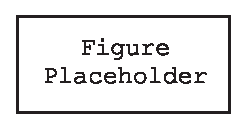
\includegraphics[width=4.6in]{c_cil0/uintrep1.eps}
\caption{Representation Of Unsigned Machine Integers}
\label{fig:ccil0:sroi0:srou0:00}
\end{figure}

\begin{equation}
\label{eq:ccil0:sroi0:srou0:00}
u = \sum_{i=0}^{m-1} u_{[i]} 2^i .
\end{equation}

In general, an $m$-bit unsigned integer can assume the values of 
0 through $2^m - 1$, so that

\begin{equation}
\label{eq:ccil0:sroi0:srou0:01}
u \in \{0, \ldots{} , 2^m - 1 \} .
\end{equation}

Unsigned synthetic long integers are always represented as an array
of unsigned machine integers.  
Consistent with the GMP \cite{bibref:s:gnumultipleprecisionarithmeticlibrary},
we call each element of the array a \emph{limb} and we call the size of
each limb the \emph{limbsize}.  This usage is very close to what Knuth
calls the \emph{word}size $w$ in the excerpt presented in 
Section \ref{ccil0:sppm0:smas0}.

Microcontroller processors are more likely than more powerful processors to have
a non-orthogonal instruction set, and so the limbsize may not be consistent between
operations in an arithmetic library.
With some processors, the appropriate limbsize may vary depending on the operation being
performed.  
For example, a microcontroller processor may be able to add two 16-bit integers to
obtain a 16-bit result plus a carry, but only be able to multiply two 8-bit integers to 
obtain a 16-bit result (thus, the appropriate limbsize for addition may be 
16 bits while the appropriate limbsize for multiplication may be 8 bits).
In such cases, it is usually most efficient to add using 16-bit limbs but
multiply using 8-bit limbs.  Adding using 8-bit limbs on a machine which will
support 16-bit additions is not normally a good design decision---even if the 
machine supports an 8-bit addition instruction which is faster than the 16-bit addition
instruction, $m/2$ 16-bit additions will nearly always be faster than 
$m$ 8-bit additions.  Using different limbsizes within the same arithmetic library
may require some consideration of alignment and 
endian issues, but these are implementation details
which are easily solved.

We view a synthetic long unsigned integer as an array of limbs (machine integers)
of some size, and we agree that we will not address the array in any other way than
by loading and storing limbs of this size.\footnote{Well \ldots{} not quite.
In software for large computers (personal computers and workstations) with an
orthogonal instruction set, we may be able to adhere to this rule.  However,
with microcontrollers, arithmetic libraries which are optimized
may break this rule.}  In particular, because
computers may be ``big-endian'' or ``little-endian'', loading and storing 
smaller units than limbs may lead in
a worst case to software defects or in a best case to non-portable code.

Assume that $w$ is the number of bits in a limb.
Notationally, we denote an unsigned
synthetic long integer as an array of $m$ limbs
$u_{m-1}$ through $u_0$, each containing $w$ bits,
with $u_0$ the least significant machine integer.  
We may also define $b=2^w$ (consistent with Knuth's
notation).
The value of
such a synthetic long machine integer is

\begin{equation}
\label{eq:ccil0:sroi0:srou0:02}
u = \sum_{i=0}^{m-1} u_{i} 2^{wi} 
=
\sum_{i=0}^{m-1} u_{i} b^i.
\end{equation}

As an alternative, we may write the value as the sum of the bit-values,

\begin{equation}
\label{eq:ccil0:sroi0:srou0:03}
u = \sum_{i=0}^{wm-1} u_{[i]} 2^{i} .
\end{equation}

Naturally, the range of such a synthetic long integer is

\begin{equation}
\label{eq:ccil0:sroi0:srou0:04}
u \in \{0, \ldots{} , 2^{wm} - 1 \} .
\end{equation}

In storing an unsigned synthetic long machine integer, the most natural way
to order the array of limbs depends on whether dynamic memory allocation is
used by the arithmetic library.  In microcontroller work, where arithmetic
library subroutines typically operate on fixed-size operands and produce
fixed-size results, storing 
limbs most significant limb first (i.e. in `C', so that element \texttt{[0]}
of the array of limbs contains the most significant limb) may be natural
and convenient.  However, this ordering would lead to computational waste in a library such
as the GMP \cite{bibref:s:gnumultipleprecisionarithmeticlibrary} where integers
may grow arbitrarily large and the library may need to reallocate long synthetic
integers to contain more limbs, as each reallocation would need to be followed
by a memory copy to align the integer's existing limbs to the end of the array.
For libraries such as the GMP, it is more practical to store limbs 
least-significant limb first, as it eliminates the need to copy memory 
when reallocations are done.



%%%%%%%%%%%%%%%%%%%%%%%%%%%%%%%%%%%%%%%%%%%%%%%%%%%%%%%%%%%%%%%%%%%%%%%%%%
%%%%%%%%%%%%%%%%%%%%%%%%%%%%%%%%%%%%%%%%%%%%%%%%%%%%%%%%%%%%%%%%%%%%%%%%%%
%%%%%%%%%%%%%%%%%%%%%%%%%%%%%%%%%%%%%%%%%%%%%%%%%%%%%%%%%%%%%%%%%%%%%%%%%%
\subsection{Representation Of Signed Integers}
%Subsection Tag: ROS0
\label{ccil0:sroi0:sros0}

Signed machine integers are always represented in two's complement form on modern
processors.  This representation is universal because of the digital logic 
conveniences---the same addition and subtraction mappings which are correct 
for unsigned machine integers are also correct for signed machine integers, 
although the criteria for overflow and comparison are
different.

Most readers are familiar with two's complement representation, so we will not
belabor it.  However, we will present essential properties.
When two's complement representation is used in an $m$-bit machine integer $u$:

\begin{enumerate}
\item All bit patterns with $u_{[m-1]} = 0$ represent non-negative integers, and 
      represent the same integer as if the representation were unsigned.
\item All bit patterns with $u_{[m-1]} = 1$ represent negative numbers; specifically
      $u_{[m-2:0]} - 2^{m-1}$; i.e.

      \begin{equation}
      \label{eq:ccil0:sroi0:sros0:00}
      u = - u_{[m-1]} 2^{m-1} + \sum_{i=0}^{m-2} u_{[i]} 2^i .
      \end{equation}

\item $u \in \{-2^{m-1}, \ldots{}, 2^{m-1}-1 \}$.
\item All bit patterns represent a unique integer.
\item For any integer except $-2^{m-1}$, 
      negation can be performed by forming the one's complement (complementing
      every bit), then adding one.  To see why this is true algebraically, note that

\end{enumerate}


However, let us observe that the value of an
$m$-bit two's complement
machine integer is


In general, an $m$-bit signed machine integer can assume the values of 
$-2^{m-1}$ through $2^{m-1} - 1$, so that

\begin{equation}
\label{eq:ccil0:sroi0:sros0:01}
u \in \{-2^{m-1}, \ldots{} , 2^{m-1} - 1 \} .
\end{equation}

There are [at least] two different representations of signed 
multiple-precision integers:

\begin{itemize}
\item Two's complement representation.
\item Sign-magnitude representation.
\end{itemize}

There are two different representations commonly used 
for signed multiple-precision integers because two's complement
representation is not ideal for multiplication and division, although
it is ideal for addition and subtraction.  For multiple-precision
integer arithmetic, sign-magnitude representation is more common.

In two's complement representation of multiple-precision integers,
the representation is the same as suggested by 
(\ref{eq:ccil0:sroi0:sros0:00}), except
more bits are involved.  For a two's complement representation
of a number consisting of $n$ machine integers with $W$ bits per
machine integer,

\begin{equation}
\label{eq:ccil0:sroi0:sros0:02}
u = - u_{B(Wn-1)} 2^{Wn-1} + \sum_{i=0}^{Wn-2} u_{B(i)} 2^i .
\end{equation}

Because we would like to know how to compare signed multiple-precision
integers in two's complement representation, we can gain some
insight into the representation by rewriting 
(\ref{eq:ccil0:sroi0:sros0:02}) in terms of machine integers:

\begin{equation}
\label{eq:ccil0:sroi0:sros0:03}
u = - u_{B(Wn-1)} 2^{Wn-1} 
+ 
\sum_{i=W(m-1)}^{Wn-2} u_{B(i)} 2^i 
+
\sum_{i=0}^{m-2} u_{i} 2^{Wi} .
\end{equation}

(\ref{eq:ccil0:sroi0:sros0:03}) gives some insight into the
relative values of multiple-precision signed two's complement
integers with respect to the values of the machine integers
that comprise them.  We discuss this further in
Section \ref{ccil0:scsi0}.

In sign-magnitude representation of multiple-precision signed two's
complement integers, an integer $u$ is represented as a sign
bit (usually a value of one indicates negativity), and a magnitude, 
which is $|u|$.  Unlike two's complement representation,
sign-magnitude representation, has two representations of zero---a positive
one and a negative one.  Either a canonical form for zero should be
adopted, or both values should be treated identically.

Assuming that the sign bit is stored in the most significant bit position,
it is easy to deduce that the value of a multiple-precision
signed two's complement integer in sign-magnitude representation is

\begin{equation}
\label{eq:ccil0:sros0:srou0:04}
u = (-1)^{u_{B(m-1)}} \sum_{i=0}^{m-2} u_{B(i)} 2^i .
\end{equation}

Sign-magnitude representation is especially convenient because
it allows machine instructions which accept unsigned operands to be used
to make calculations involving signed integers.



%%%%%%%%%%%%%%%%%%%%%%%%%%%%%%%%%%%%%%%%%%%%%%%%%%%%%%%%%%%%%%%%%%%%%%%%%%
%%%%%%%%%%%%%%%%%%%%%%%%%%%%%%%%%%%%%%%%%%%%%%%%%%%%%%%%%%%%%%%%%%%%%%%%%%
%%%%%%%%%%%%%%%%%%%%%%%%%%%%%%%%%%%%%%%%%%%%%%%%%%%%%%%%%%%%%%%%%%%%%%%%%%
\section{Characteristics Of Practical Processors}
%Section tag: CPP
\label{ccil0:scpp0}

Before discussing specific algorithms, it is necessary to 
discuss the construction of practical processors---how such a processor
manipulates machine integers.  We accept as a typical processor the
TMS-370C8, an 8-bit microcontroller manufactured by 
Texas Instruments.

\begin{figure}
\centering
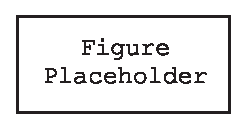
\includegraphics[width=4.6in]{c_cil0/t370flag.eps}
\caption{Texas Instruments TMS-370C8 Flags}
\label{fig:ccil0:scpp0:00}
\end{figure}

\begin{figure}
\centering
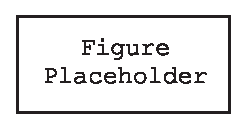
\includegraphics[width=4.6in]{c_cil0/t370cjmp.eps}
\caption{Texas Instruments TMS-370C8 Conditional Jump Instructions}
\label{fig:ccil0:scpp0:01}
\end{figure}

A typical microcontroller allows operations on machine integers
in the following steps:

\begin{itemize}
\item A machine instruction is performed on one or two machine 
      integer operands (for example:  addition, subtraction, 
      multiplication, division, increment, decrement, complement,
      negation, or comparison).  This machine instruction may
      produce a result, and usually sets a number of condition flags that
      reflect the nature and validity of the result (Is it zero?
      Is it negative?  Did the result overflow?).  As an
      example, the condition
      flags of the TMS-370C8 are shown in Figure \ref{fig:ccil0:scpp0:00}.
      .
\item A conditional branch instruction is used to branch conditionally
      based on the state of the condition flags.  The definition of
      the condition flags and the way in which the conditional
      branch instruction utilizes them is designed to provide a
      way to treat both unsigned and signed machine integers.
      As an example, the way in which the conditional
      jump instructions of the TMS-370C8 use the flags
      is shown in Figure \ref{fig:ccil0:scpp0:01}.
\end{itemize}

It is not too often necessary to understand in detail
the Boolean relationships that govern how machine integers are
added, subtracted, and compared; and how signed comparisons differ
from unsigned comparisons.  In most cases, it is adequate to
rely on the design of the microcontroller.  However, we do present
rudimentary observations in this section.



%%%%%%%%%%%%%%%%%%%%%%%%%%%%%%%%%%%%%%%%%%%%%%%%%%%%%%%%%%%%%%%%%%%%%%%%%%
%%%%%%%%%%%%%%%%%%%%%%%%%%%%%%%%%%%%%%%%%%%%%%%%%%%%%%%%%%%%%%%%%%%%%%%%%%
%%%%%%%%%%%%%%%%%%%%%%%%%%%%%%%%%%%%%%%%%%%%%%%%%%%%%%%%%%%%%%%%%%%%%%%%%%
\section{Comparison Of Integers}


%%%%%%%%%%%%%%%%%%%%%%%%%%%%%%%%%%%%%%%%%%%%%%%%%%%%%%%%%%%%%%%%%%%%%%%%%%
%%%%%%%%%%%%%%%%%%%%%%%%%%%%%%%%%%%%%%%%%%%%%%%%%%%%%%%%%%%%%%%%%%%%%%%%%%
%%%%%%%%%%%%%%%%%%%%%%%%%%%%%%%%%%%%%%%%%%%%%%%%%%%%%%%%%%%%%%%%%%%%%%%%%%
\subsection{Comparison Of Unsigned Integers}


%%%%%%%%%%%%%%%%%%%%%%%%%%%%%%%%%%%%%%%%%%%%%%%%%%%%%%%%%%%%%%%%%%%%%%%%%%
%%%%%%%%%%%%%%%%%%%%%%%%%%%%%%%%%%%%%%%%%%%%%%%%%%%%%%%%%%%%%%%%%%%%%%%%%%
%%%%%%%%%%%%%%%%%%%%%%%%%%%%%%%%%%%%%%%%%%%%%%%%%%%%%%%%%%%%%%%%%%%%%%%%%%
\subsection{Comparison Of Signed Integers}
%Section Tag: CSI0
\label{ccil0:scsi0}


%%%%%%%%%%%%%%%%%%%%%%%%%%%%%%%%%%%%%%%%%%%%%%%%%%%%%%%%%%%%%%%%%%%%%%%%%%
%%%%%%%%%%%%%%%%%%%%%%%%%%%%%%%%%%%%%%%%%%%%%%%%%%%%%%%%%%%%%%%%%%%%%%%%%%
%%%%%%%%%%%%%%%%%%%%%%%%%%%%%%%%%%%%%%%%%%%%%%%%%%%%%%%%%%%%%%%%%%%%%%%%%%
\section{Integer Addition}
%Section tag: IAD0
\label{ccil0:siad0}

Addition of two $m$-bit integers is a combinational function---that is,
the inputs uniquely determine the output.  Addition of binary 
numbers is performed 


%%%%%%%%%%%%%%%%%%%%%%%%%%%%%%%%%%%%%%%%%%%%%%%%%%%%%%%%%%%%%%%%%%%%%%%%%%
%%%%%%%%%%%%%%%%%%%%%%%%%%%%%%%%%%%%%%%%%%%%%%%%%%%%%%%%%%%%%%%%%%%%%%%%%%
%%%%%%%%%%%%%%%%%%%%%%%%%%%%%%%%%%%%%%%%%%%%%%%%%%%%%%%%%%%%%%%%%%%%%%%%%%
\subsection{Hardware Implementation Of Addition}


%%%%%%%%%%%%%%%%%%%%%%%%%%%%%%%%%%%%%%%%%%%%%%%%%%%%%%%%%%%%%%%%%%%%%%%%%%
%%%%%%%%%%%%%%%%%%%%%%%%%%%%%%%%%%%%%%%%%%%%%%%%%%%%%%%%%%%%%%%%%%%%%%%%%%
%%%%%%%%%%%%%%%%%%%%%%%%%%%%%%%%%%%%%%%%%%%%%%%%%%%%%%%%%%%%%%%%%%%%%%%%%%
\subsection{Addition Of Unsigned Operands}


%%%%%%%%%%%%%%%%%%%%%%%%%%%%%%%%%%%%%%%%%%%%%%%%%%%%%%%%%%%%%%%%%%%%%%%%%%
%%%%%%%%%%%%%%%%%%%%%%%%%%%%%%%%%%%%%%%%%%%%%%%%%%%%%%%%%%%%%%%%%%%%%%%%%%
%%%%%%%%%%%%%%%%%%%%%%%%%%%%%%%%%%%%%%%%%%%%%%%%%%%%%%%%%%%%%%%%%%%%%%%%%%
\subsection{Addition Of Signed Operands}


%%%%%%%%%%%%%%%%%%%%%%%%%%%%%%%%%%%%%%%%%%%%%%%%%%%%%%%%%%%%%%%%%%%%%%%%%%
%%%%%%%%%%%%%%%%%%%%%%%%%%%%%%%%%%%%%%%%%%%%%%%%%%%%%%%%%%%%%%%%%%%%%%%%%%
%%%%%%%%%%%%%%%%%%%%%%%%%%%%%%%%%%%%%%%%%%%%%%%%%%%%%%%%%%%%%%%%%%%%%%%%%%
\section {Integer Subtraction}


%%%%%%%%%%%%%%%%%%%%%%%%%%%%%%%%%%%%%%%%%%%%%%%%%%%%%%%%%%%%%%%%%%%%%%%%%%
%%%%%%%%%%%%%%%%%%%%%%%%%%%%%%%%%%%%%%%%%%%%%%%%%%%%%%%%%%%%%%%%%%%%%%%%%%
%%%%%%%%%%%%%%%%%%%%%%%%%%%%%%%%%%%%%%%%%%%%%%%%%%%%%%%%%%%%%%%%%%%%%%%%%%
\subsection{Hardware Implementation Of Subtraction}


%%%%%%%%%%%%%%%%%%%%%%%%%%%%%%%%%%%%%%%%%%%%%%%%%%%%%%%%%%%%%%%%%%%%%%%%%%
%%%%%%%%%%%%%%%%%%%%%%%%%%%%%%%%%%%%%%%%%%%%%%%%%%%%%%%%%%%%%%%%%%%%%%%%%%
%%%%%%%%%%%%%%%%%%%%%%%%%%%%%%%%%%%%%%%%%%%%%%%%%%%%%%%%%%%%%%%%%%%%%%%%%%
\subsection{Subtraction Of Unsigned Operands}


%%%%%%%%%%%%%%%%%%%%%%%%%%%%%%%%%%%%%%%%%%%%%%%%%%%%%%%%%%%%%%%%%%%%%%%%%%
%%%%%%%%%%%%%%%%%%%%%%%%%%%%%%%%%%%%%%%%%%%%%%%%%%%%%%%%%%%%%%%%%%%%%%%%%%
%%%%%%%%%%%%%%%%%%%%%%%%%%%%%%%%%%%%%%%%%%%%%%%%%%%%%%%%%%%%%%%%%%%%%%%%%%
\subsection{Subtraction Of Signed Operands}



%%%%%%%%%%%%%%%%%%%%%%%%%%%%%%%%%%%%%%%%%%%%%%%%%%%%%%%%%%%%%%%%%%%%%%%%%%
%%%%%%%%%%%%%%%%%%%%%%%%%%%%%%%%%%%%%%%%%%%%%%%%%%%%%%%%%%%%%%%%%%%%%%%%%%
%%%%%%%%%%%%%%%%%%%%%%%%%%%%%%%%%%%%%%%%%%%%%%%%%%%%%%%%%%%%%%%%%%%%%%%%%%
\section{Integer Multiplication}


%%%%%%%%%%%%%%%%%%%%%%%%%%%%%%%%%%%%%%%%%%%%%%%%%%%%%%%%%%%%%%%%%%%%%%%%%%
%%%%%%%%%%%%%%%%%%%%%%%%%%%%%%%%%%%%%%%%%%%%%%%%%%%%%%%%%%%%%%%%%%%%%%%%%%
%%%%%%%%%%%%%%%%%%%%%%%%%%%%%%%%%%%%%%%%%%%%%%%%%%%%%%%%%%%%%%%%%%%%%%%%%%
\subsection{Hardware Implementation Of Multiplication}


%%%%%%%%%%%%%%%%%%%%%%%%%%%%%%%%%%%%%%%%%%%%%%%%%%%%%%%%%%%%%%%%%%%%%%%%%%
%%%%%%%%%%%%%%%%%%%%%%%%%%%%%%%%%%%%%%%%%%%%%%%%%%%%%%%%%%%%%%%%%%%%%%%%%%
%%%%%%%%%%%%%%%%%%%%%%%%%%%%%%%%%%%%%%%%%%%%%%%%%%%%%%%%%%%%%%%%%%%%%%%%%%
\subsection{Multiplication Of Unsigned Operands}


%%%%%%%%%%%%%%%%%%%%%%%%%%%%%%%%%%%%%%%%%%%%%%%%%%%%%%%%%%%%%%%%%%%%%%%%%%
%%%%%%%%%%%%%%%%%%%%%%%%%%%%%%%%%%%%%%%%%%%%%%%%%%%%%%%%%%%%%%%%%%%%%%%%%%
%%%%%%%%%%%%%%%%%%%%%%%%%%%%%%%%%%%%%%%%%%%%%%%%%%%%%%%%%%%%%%%%%%%%%%%%%%
\subsection{Multiplication Of Signed Operands}



%%%%%%%%%%%%%%%%%%%%%%%%%%%%%%%%%%%%%%%%%%%%%%%%%%%%%%%%%%%%%%%%%%%%%%%%%%
%%%%%%%%%%%%%%%%%%%%%%%%%%%%%%%%%%%%%%%%%%%%%%%%%%%%%%%%%%%%%%%%%%%%%%%%%%
%%%%%%%%%%%%%%%%%%%%%%%%%%%%%%%%%%%%%%%%%%%%%%%%%%%%%%%%%%%%%%%%%%%%%%%%%%
\section{Integer Division}
\label{ccil0:sidv0}

\index{division}\index{integer division}In this section,
we discuss the best known methods of dividing integers using
typical microcontroller instruction sets.  In general, given
two arbitrary integers $p$ and $q$, we are interested in determining
their quotient $q=\lfloor{}p/q\rfloor$ and remainder
$r=p\bmod{}q$ as economically as possible.


%%%%%%%%%%%%%%%%%%%%%%%%%%%%%%%%%%%%%%%%%%%%%%%%%%%%%%%%%%%%%%%%%%%%%%%%%%
%%%%%%%%%%%%%%%%%%%%%%%%%%%%%%%%%%%%%%%%%%%%%%%%%%%%%%%%%%%%%%%%%%%%%%%%%%
%%%%%%%%%%%%%%%%%%%%%%%%%%%%%%%%%%%%%%%%%%%%%%%%%%%%%%%%%%%%%%%%%%%%%%%%%%
\subsection{Hardware Implementation Of Division}


%%%%%%%%%%%%%%%%%%%%%%%%%%%%%%%%%%%%%%%%%%%%%%%%%%%%%%%%%%%%%%%%%%%%%%%%%%
%%%%%%%%%%%%%%%%%%%%%%%%%%%%%%%%%%%%%%%%%%%%%%%%%%%%%%%%%%%%%%%%%%%%%%%%%%
%%%%%%%%%%%%%%%%%%%%%%%%%%%%%%%%%%%%%%%%%%%%%%%%%%%%%%%%%%%%%%%%%%%%%%%%%%
\subsection{General Unsigned Division Without A Machine Division Instruction}
\label{ccil0:sidv0:sgdn0}


%%%%%%%%%%%%%%%%%%%%%%%%%%%%%%%%%%%%%%%%%%%%%%%%%%%%%%%%%%%%%%%%%%%%%%%%%%
%%%%%%%%%%%%%%%%%%%%%%%%%%%%%%%%%%%%%%%%%%%%%%%%%%%%%%%%%%%%%%%%%%%%%%%%%%
%%%%%%%%%%%%%%%%%%%%%%%%%%%%%%%%%%%%%%%%%%%%%%%%%%%%%%%%%%%%%%%%%%%%%%%%%%
\subsection{General Unsigned Division With A Machine Division Instruction}
\label{ccil0:sidv0:sgdu0}

As mentioned many places in this work, efficiency in microcontroller software
involves phrasing computational problems in a way which makes good use of
the machine instruction set.  In Section \ref{ccil0:sidv0:sgdn0} we discussed
the classic shift-compare-subtract algorithm for division.  This algorithm
is far from efficient.  A reasonable question to ask is whether we can
leverage ``small'' division capability (provided by the machine instruction set)
to accomplish ``large'' divisions (those which we require in practice).
It ends up that this is possible:  the technique involved is effectively
to use machine division instructions to estimate the highest-order bits of 
the quotient based on the highest-order bits of the dividend and divisor.

Knuth's discussion of division 
algorithms \cite[pp. 270-275]{bibref:b:knuthclassic2ndedvol2} is the
basis for most of the material in this subsection.  However, Knuth has
a gift for terseness that is sometimes a curse for the reader, and so
we take more time than Knuth to explain certain results.

First, as a starting point, we present \emph{Algorithm D} from
Knuth \cite[pp. 272-273]{bibref:b:knuthclassic2ndedvol2}.  Then,
we justify the algorithm and explain why it is valid.  Finally,
we supply implementation advice for microcontroller instruction sets.

\begin{vworkalgorithmstatementpar}{Arbitrary Unsigned Division Using 
Machine Unsigned Division Instructions}
\label{alg:ccil0:sidv0:sgdu0:01}
(From Knuth \cite[pp. 272-273]{bibref:b:knuthclassic2ndedvol2})
Given nonnegative integers $u=(u_{m+n-1} \ldots{} u_1 u_0)_b$
and $v=(v_{n-1} \ldots{} v_1 v_0)_b$, where
$v_{n-1} \neq 0$ and $n > 1$, we form the radix-$b$ quotient
$\lfloor{}u/v\rfloor{} = (q_m q_{m-1} \ldots{} q_0)_b$ and
the remainder $u \bmod v = (r_{n-1} \ldots{} r_1 r_0)_b$.  When
$n=1$, the simpler algorithm of 
Subsection \ref{ccil0:sidv0:sldm0}
should be used. 

\begin{algblvl0}
\item \label{enumstep:alg:ccil0:sidv0:sgdu0:01:01}
      [Normalize.] Set $d \gets \lfloor{}b/(v_{n-1} + 1)\rfloor$.
      Then set $(u_{m+n} u_{m+n-1} \ldots{} u_1 u_0)_b$ equal to 
      $(u_{m+n-1} \ldots{} u_1 u_0)_b$ times $d$; similarly,
      set $(v_{n-1} \ldots{} v_1 v_0)_b$ equal to 
      $(v_{n-1} \ldots{} v_1 v_0)_b$ times $d$.  (Notice the introduction
      of a new digit position $u_{m+n}$ at the left of
      $u_{m+n-1}$; if $d=1$, all we need to do in this step is set
      $u_{m+n} \gets 0$.  On a binary computer it may be preferable
      to choose $d$ to be a power of 2 instead of using the value
      suggested here; any value of $d$ that results in
      $v_{n-1} \geq \lfloor{}b/2\rfloor$ will suffice.  See also
      exercise 37.)
\item \label{enumstep:alg:ccil0:sidv0:sgdu0:01:02}
      [Initialize $j$.]  Set $j \gets m$.  (The loop on $j$,
      steps 
      \ref{enumstep:alg:ccil0:sidv0:sgdu0:01:03} 
      through 
      \ref{enumstep:alg:ccil0:sidv0:sgdu0:01:07}, 
      will be essentially a division of 
      $(u_{j+n} \ldots{} u_{j+1} u_j)_b$ by $(v_{n-1} \ldots{} v_1 v_0)_b$ to
      get a single quotient digit $q_j$; see Figure \ref{fig:alg:ccil0:sidv0:sgdu0:01:01}.)

\begin{figure}
\centering
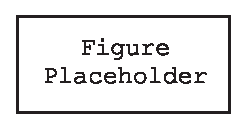
\includegraphics[width=4.6in]{c_cil0/kdfc01.eps}
\caption{Flowchart For Algorithm \ref{alg:ccil0:sidv0:sgdu0:01} (From \cite[p. 273]{bibref:b:knuthclassic2ndedvol2})}
\label{fig:alg:ccil0:sidv0:sgdu0:01:01}
\end{figure}

\item \label{enumstep:alg:ccil0:sidv0:sgdu0:01:03}
      [Calculate $\hat{q}$.]  Set
      $\hat{q} \gets \lfloor{}u_{j+n}b + u_{j+n-1})/v_{n-1}\rfloor$ and
      let $\hat{r}$ be the remainder, $(u_{j+n}b + u_{j+n-1}) \bmod v_{n-1}$.
      Now test if $\hat{q} = b$ or $\hat{q} v_{n-2} > b\hat{r} + u_{j+n-2}$;
      if so, decrease $\hat{q}$ by 1, increase $\hat{r}$ by $v_{n-1}$, and repeat
      this test if $\hat{r} < b$.  (The test of $v_{n-2}$ determines at high
      speed most of the cases in which the trial value $\hat{q}$ is one too large,
      and it eliminates \emph{all} cases where $\hat{q}$ is two too large;
      see exercises 19, 20, 21.)
\item \label{enumstep:alg:ccil0:sidv0:sgdu0:01:04}
      [Multiply and subtract.]  Replace $(u_{j+n} u_{j+n-1} \ldots{} u_j)_b$ by

      \begin{equation}
      \nonumber
      (u_{j+n} u_{j+n-1} \ldots{} u_j)_b - \hat{q} (0 v_{n-1} \ldots{} v_1 v_0)_b. 
      \end{equation}

      This computation consists of a simple multiplication by a one-place number,
      combined with a subtraction.  The digits $(u_{j+n}, u_{j+n-1}, \ldots{}, u_j)$
      should be kept positive; if the result of this step is actually negative, 
      $(u_{j+n} u_{j+n-1} \ldots{} u_j)_b$ should be left as the true
      value plus $b^{n+1}$, namely as the $b$'s complement of the true value, and 
      a ``borrow'' to the left should be remembered.
\item \label{enumstep:alg:ccil0:sidv0:sgdu0:01:05}
      [Test remainder.]  Set $q_j \gets \hat{q}$.  If the result of step 
      \ref{enumstep:alg:ccil0:sidv0:sgdu0:01:04} was negative, go to
      step \ref{enumstep:alg:ccil0:sidv0:sgdu0:01:06}; otherwise go on to
      step \ref{enumstep:alg:ccil0:sidv0:sgdu0:01:07}.
\item \label{enumstep:alg:ccil0:sidv0:sgdu0:01:06}
      [Add back.]  (The probability that this step is necessary is very small, on the 
      order of only $2/b$, as shown in exercise 21; test data to activate this step
      should therefore be specifically contrived when debugging.)  Decrease 
      $q_j$ by 1, and add $(0 v_{n-1} \ldots v_1 v_0)_b$ to
      $(u_{j+n} u_{j+n-1} \ldots{} u_{j+1} u_j)_b$.  (A carry will occur to the left of
      $u_{j+n}$, and it should be ignored since it cancels with the borrow that
      occured in step \ref{enumstep:alg:ccil0:sidv0:sgdu0:01:04}.) 
\item \label{enumstep:alg:ccil0:sidv0:sgdu0:01:07}
      [Loop on $j$.]  Decrease $j$ by one.  Now if $j \geq 0$, go back to step
      \ref{enumstep:alg:ccil0:sidv0:sgdu0:01:03}.
\item \label{enumstep:alg:ccil0:sidv0:sgdu0:01:08}
      [Unnormalize.]  Now $(q_m \ldots{} q_1 q_0)_b$ is the desired quotient, and
      the desired remainder may be obtained by dividing 
      $(u_{n-1} \ldots{} u_1 u_0)_b$ by $d$.
\end{algblvl0}
\end{vworkalgorithmstatementpar}
\vworkalgorithmfooter{}

The general idea of Algorithm \ref{alg:ccil0:sidv0:sgdu0:01} is that 
digits (machine words) of the quotient $q$ can be successively estimated 
based on the first digits of the dividend and divisor.  Knuth
\cite[p. 271]{bibref:b:knuthclassic2ndedvol2} explores the properties of
the digit estimate 

\begin{equation}
\label{eq:ccil0:sidv0:sgdu0:01}
\hat{q} = \min \left( {\left\lfloor{\frac{u_n b + u_{n-1}}{v_{n-1}}}\right\rfloor, b-1} \right).
\end{equation}

The first point to make about an estimate in the form of 
(\ref{eq:ccil0:sidv0:sgdu0:01}) is that it can only be accomplished
efficiently if the machine-native division instruction supports
overflow detection, since it is possible that
$(u_n b + u_{n-1})/v_{n-1} \geq b$, even if 
$u/v < b$, as is shown by the following example.

\begin{vworkexamplestatement}
\label{ex:ccil0:sidv0:sgdu0:01:01}
Assume that we wish to apply the estimate of $\hat{q}$ provided by 
(\ref{eq:ccil0:sidv0:sgdu0:01})
to $u=16,776,704$ and $v=65,535$.  Demonstrate that a machine division
overflow will occur when estimating the first digit, assuming a processor
that can divide a 16-bit dividend by an 8-bit divisor to produce an 8-bit
quotient.
\end{vworkexamplestatement}
\begin{vworkexampleparsection}{Solution}
Note that according to Knuth's intention, the word size on such a machine
is 8 bits.  Thus, $b=256$.  Note that $u/v = 255 + 255/256 < b = 256$, as
required by Knuth's precondition.  However, although $u/v < b$, 
$u = [255 \; 254 \; 0] [256^2 \; 256 \; 1]^T = [u_2 u_1 u_0] [b^2 b^1 b^0]^T$ and 
$v = [255 \; 255] [256 \; 1]^T = [v_1 v_0] [b^1 b^0]^T$, so that calculating
an estimate $\hat{q}$ as required by (\ref{eq:ccil0:sidv0:sgdu0:01}),
$(u_n b + u_{n-1})/v_{n-1} = 65,534/255 = 256 + 254/255 \geq b$, is a division
overflow for a single machine division instruction.  Thus, it follows that 
a machine with division overflow detection can quickly determine that $b-1$ from
(\ref{eq:ccil0:sidv0:sgdu0:01}) is the minimum, whereas a machine without 
division overflow
detection would have to use several additional machine instructions to make
this determination.
\end{vworkexampleparsection}
\vworkexamplefooter{}

The second thing to establish about $\hat{q}$ as defined by 
(\ref{eq:ccil0:sidv0:sgdu0:01}) is how ``good'' of an estimate 
$\hat{q}$ is---how much information, exactly, about $q$ can we
obtain by examining the first two words of $u$ and the first
word of $v$?

We first establish in the following lemma that our estimate of
$q$, $\hat{q}$, can be no less than $q$.

\begin{vworklemmastatementpar}{\mbox{\boldmath$\hat{q} \geq q$}}
\label{lem:ccil0:sidv0:sgdu0:01}
The estimate of $q$ provided by (\ref{eq:ccil0:sidv0:sgdu0:01}),
$\hat{q}$ is always at least as great as the actual value of 
$q$, i.e. $\hat{q} \geq q$.
\end{vworklemmastatementpar}
\begin{vworklemmaproof}
Knowledge of $u_{n}$, $u_{n-1}$, and $v_{n-1}$ necessarily confine
the intervals in which the actual values of $u$ and $v$ may be;
specifically:\footnote{In
(\ref{eq:lem:ccil0:sidv0:sgdu0:01:04})
and 
(\ref{eq:lem:ccil0:sidv0:sgdu0:01:07}),
we use statements of the form ``$x = x$'' as an idiom for
``$x$ is known''.}

\begin{eqnarray}
\label{eq:lem:ccil0:sidv0:sgdu0:01:01}
u & = & \sum_{i=0}^{n} u_i b^i   \\
\label{eq:lem:ccil0:sidv0:sgdu0:01:02}
  & = & u_n b^n + u_{n-1} b^{n-1} + \ldots{} + u_2 b^2 + u_1 b + u_0   \\
\label{eq:lem:ccil0:sidv0:sgdu0:01:03}
  & = & (u_n b + u_{n-1}) b^{n-1} + \ldots{} + u_2 b^2 + u_1 b + u_0
\end{eqnarray}

\begin{eqnarray}
\nonumber & (u_n = u_n \wedge u_{n-1} = u_{n-1}) & \\
\label{eq:lem:ccil0:sidv0:sgdu0:01:04}
& \vworkvimp & \\
\nonumber & (u_n b + u_{n-1}) b^{n-1} \leq u \leq (u_n b + u_{n-1}) b^{n-1} + b^{n-1} - 1 &
\end{eqnarray}

\begin{eqnarray}
\label{eq:lem:ccil0:sidv0:sgdu0:01:05}
v & = & \sum_{i=0}^{n-1} v_i b^i   \\
\label{eq:lem:ccil0:sidv0:sgdu0:01:06}
& = & v_{n-1} b^{n-1} + v_{n-2} b^{n-2} + \ldots{} + v_2 b^2 + v_1 b + v_0 
\end{eqnarray}

\begin{equation}
\label{eq:lem:ccil0:sidv0:sgdu0:01:07}
(v_{n-1} = v_{n-1})
\vworkhimp
v_{n-1} b^{n-1} \leq v \leq v_{n-1} b^{n-1} + b^{n-1} - 1 
\end{equation}

(\ref{eq:lem:ccil0:sidv0:sgdu0:01:04}) and
(\ref{eq:lem:ccil0:sidv0:sgdu0:01:07}) reflect the uncertainties in the 
values of $u$ and $v$ respectively because only the first digit(s) of
$u$ and $v$ are being considered in forming the estimate $\hat{q}$.

By definition, the actual value of $q$ is $\lfloor{}u/v\rfloor$.  For a 
rational function $f(u,v) = u/v$ where $u \in [u_{min}, u_{max}]$ and
$v \in [v_{min}, v_{max}]$, the minimum value of $u/v$ occurs at 
$u_{min}/v_{max}$, and the maximum value of $u/v$ occurs at
$u_{max}/v_{min}$.  We can therefore write that

\begin{equation}
\label{eq:lem:ccil0:sidv0:sgdu0:01:08}
\left\lfloor{\frac{(u_n b + u_{n-1}) b^{n-1}}{v_{n-1} b^{n-1} + b^{n-1} - 1}}\right\rfloor
\leq
q
\leq
\left\lfloor{\frac{(u_n b + u_{n-1}) b^{n-1} + b^{n-1} - 1}{v_{n-1} b^{n-1}}}\right\rfloor .
\end{equation} 

In other words, knowledge of $u_{n}$, $u_{n-1}$, and $v_{n-1}$ confines $q$ to the 
interval indicated in (\ref{eq:lem:ccil0:sidv0:sgdu0:01:08}).  We must prove that,
given a specific $u_{n}$, $u_{n-1}$, and $v_{n-1}$, $\hat{q}$ is at least as large as
the upper bound in (\ref{eq:lem:ccil0:sidv0:sgdu0:01:08}); otherwise we could find a
$q$ such that $q > \hat{q}$.  We can algebraically manipulate the upper bound in 
in (\ref{eq:lem:ccil0:sidv0:sgdu0:01:08}) to yield

\begin{equation}
\label{eq:lem:ccil0:sidv0:sgdu0:01:09}
\left\lfloor{\frac{(u_n b + u_{n-1}) b^{n-1}}{v_{n-1} b^{n-1} + b^{n-1} - 1}}\right\rfloor
\leq
q
\leq
\left\lfloor{\frac{u_n b + u_{n-1} + \frac{b^{n-1}-1}{b^{n-1}}}{v_{n-1}}}\right\rfloor .
\end{equation} 

In (\ref{eq:lem:ccil0:sidv0:sgdu0:01:09}), since $(b^{n-1}-1)/b^{n-1} < 1$ and since
$u_n b + u_{n-1}$ is an integer, we can conclude that
$\lfloor u_n b + u_{n-1} + (b^{n-1}-1)/b^{n-1} \rfloor = \lfloor u_n b + u_{n-1} \rfloor$
and hence that

\begin{equation}
\label{eq:lem:ccil0:sidv0:sgdu0:01:10}
q
\leq
\left\lfloor{\frac{u_n b + u_{n-1} + \frac{b^{n-1}-1}{b^{n-1}}}{v_{n-1}}}\right\rfloor 
=
\left\lfloor{\frac{u_n b + u_{n-1}}{v_{n-1}}}\right\rfloor 
=
\hat{q} .
\end{equation} 

Therefore, $\hat{q} \geq q$.
\end{vworklemmaproof}
\vworklemmafooter{}

Lemma \ref{lem:ccil0:sidv0:sgdu0:01} establishes that 
a digit estimate $\hat{q}$ based on the first digit of the
divisor $v$ can be no less than the actual digit $q$, i.e.
$\hat{q}-q \geq 0$.  However, we must also establish an upper bound
on $\hat{q}-q$.

Intuitively, based on
(\ref{eq:lem:ccil0:sidv0:sgdu0:01:06}), we might guess that
if $v_{n-1}$ is small, the estimate $\hat{q}$ may be quite
poor, as the interval to which the actual value of $v$ is confined
may be quite large.  This fact is the basis for the normalization
step [\ref{enumstep:alg:ccil0:sidv0:sgdu0:01:01}] in Algorithm
\ref{alg:ccil0:sidv0:sgdu0:01}.  We now prove a useful result
for how much $u, v$ must be normalized so that $\hat{q}-q \leq 2$.

\begin{vworklemmastatementpar}{Normalization Requirement So That 
                               \mbox{\boldmath$\hat{q} - q \leq 2$}}
\label{lem:ccil0:sidv0:sgdu0:02}
If $v_{n-1} \geq \lfloor b/2 \rfloor$ and $\hat{q}$ is chosen as
indicated in (\ref{eq:ccil0:sidv0:sgdu0:01}), then 
$0 \leq \hat{q} - q \leq 2$.
\end{vworklemmastatementpar}
\begin{vworklemmaproof}
The lower limit on $\hat{q} - q$ is proved in Lemma \ref{lem:ccil0:sidv0:sgdu0:01}.
We now seek only to prove that $\hat{q} - q \leq 2$.
By definition of $\hat{q}$ and $q$, 

\begin{equation}
\label{eq:lem:ccil0:sidv0:sgdu0:02:01}
\hat{q} - q  =    \left\lfloor {\frac{u_n b + u_{n-1}}{v_{n-1}}} \right\rfloor 
                  - \left\lfloor {\frac{u}{v}} \right\rfloor 
\end{equation}

When only nonnegative integers are involved, 
(\cmtnzeroxrefhyphen\ref{eq:cmtn0:sfcf0:02}) 
supplies an exact expression for the floor of a 
ratio of integers.  Using (\cmtnzeroxrefhyphen\ref{eq:cmtn0:sfcf0:02}),
(\ref{eq:lem:ccil0:sidv0:sgdu0:02:01}) can be decomposed into

\begin{equation}
\label{eq:lem:ccil0:sidv0:sgdu0:02:02}
\hat{q} - q  =    \frac{u_n b + u_{n-1}}{v_{n-1}}
                - \frac{(u_n b + u_{n-1}) \bmod v_{n-1}}{v_{n-1}}
                - \frac{u}{v}
                + \frac{u \bmod v}{v} . 
\end{equation}

\noindent{}Note that (\ref{eq:lem:ccil0:sidv0:sgdu0:02:02}) is an exact 
expression (rather than an
inequality).

Note in (\ref{eq:lem:ccil0:sidv0:sgdu0:02:02}) that
$(u_n b + u_{n-1}) \bmod v_{n-1} \in [0, v_{n-1}-1]$, and that in general
there is no reason to expect it cannot be zero.  Thus, we can assume that
it \emph{is} zero, which will maximize $\hat{q}-q$.  We can thus convert
(\ref{eq:lem:ccil0:sidv0:sgdu0:02:02}) into the inequality

\begin{equation}
\label{eq:lem:ccil0:sidv0:sgdu0:02:03}
\hat{q} - q  \leq \frac{u_n b + u_{n-1}}{v_{n-1}}
                - \frac{u}{v}
                + \frac{u \bmod v}{v} . 
\end{equation}

In (\ref{eq:lem:ccil0:sidv0:sgdu0:02:03}) we can also observe that
$(u \bmod v)/v \in [0, (v-1)/v]$.  If we replace this expression with 
``1'' (which is unattainable, but barely), this will change the relational
operator from ``$\leq$'' to ``$<$'':

\begin{equation}
\label{eq:lem:ccil0:sidv0:sgdu0:02:04}
\hat{q} - q  <    \frac{u_n b + u_{n-1}}{v_{n-1}}
                - \frac{u}{v}
                + 1 . 
\end{equation}

The result we wish to show is that with $v_{n-1} \geq \lfloor b/2 \rfloor$,
$\hat{q}-q \leq 2$.  To simplify the subsequent algebraic manipulations, note in 
(\ref{eq:lem:ccil0:sidv0:sgdu0:02:04}) that

\begin{eqnarray}
\label{eq:lem:ccil0:sidv0:sgdu0:02:05}
          & \hat{q} - q  \leq 2 &  \\    
\nonumber & \vworkvertequiv     &  \\
\label{eq:lem:ccil0:sidv0:sgdu0:02:06}
          & \displaystyle \frac{u_n b + u_{n-1}}{v_{n-1}}
                - \frac{u}{v}
                + 1 \leq 3 &          \\
\nonumber & \vworkvertequiv     &  \\
\label{eq:lem:ccil0:sidv0:sgdu0:02:07}
          & \displaystyle \frac{u_n b + u_{n-1}}{v_{n-1}}
                - \frac{u}{v} \leq 2    &
\end{eqnarray}

(\ref{eq:lem:ccil0:sidv0:sgdu0:02:06}) may be counterintuitive, so
further explanation is offered here.  Since $\hat{q} \in \vworkintset$ and $q \in \vworkintset$,
$\hat{q}-q \in \vworkintset$.  Thus, proving 
(\ref{eq:lem:ccil0:sidv0:sgdu0:02:06}) or
(\ref{eq:lem:ccil0:sidv0:sgdu0:02:07}) proves that
$\hat{q}-q \in \{ \ldots, -1, 0, 1, 2 \}$ (however, by 
Lemma \ref{lem:ccil0:sidv0:sgdu0:01}, $\hat{q}-q \geq 0$, so in fact
what would be proved is that $\hat{q}-q \in \{ 0, 1, 2 \}$).  For 
algebraic simplicity,
we choose to prove (\ref{eq:lem:ccil0:sidv0:sgdu0:02:07}).

First, adjust numerator and denominator of the first term in 
(\ref{eq:lem:ccil0:sidv0:sgdu0:02:07}) by $b^{n-1}$ so that the terms more closely 
resemble $u$ and $v$ in 
(\ref{eq:lem:ccil0:sidv0:sgdu0:01:02}) 
and 
(\ref{eq:lem:ccil0:sidv0:sgdu0:01:06}):

\begin{equation}
\label{eq:lem:ccil0:sidv0:sgdu0:02:08}
\frac{u_n b^n + u_{n-1} b^{n-1}}{v_{n-1} b^{n-1}}
                - \frac{u}{v} \leq 2 .
\end{equation}

For logical implication to be maintained,
we must make the most pessimistic choices and assumptions possible in 
(\ref{eq:lem:ccil0:sidv0:sgdu0:02:08}) in order to maximize the value
of the left side of the inequality.
The first assumption to be made is the error in estimating
$u$ and $v$ based on their most significant digits.  It can be
seen that (\ref{eq:lem:ccil0:sidv0:sgdu0:02:08}) will be maximized if:

\begin{itemize}
\item We assume that $u = u_{n} b^n + u_{n-1} b^{n-1}$ (i.e. that we estimate
      $u$ precisely).
\item We assume that $v = v_{n-1} b^{n-1} + b^{n-1} - 1$ (i.e. that
      we underestimate $v$ by the maximum amount possible).
\item We minimize the value of $v_{n-1} b^{n-1}$.
\end{itemize}

Assuming that $u$ is estimated precisely yields

\begin{equation}
\label{eq:lem:ccil0:sidv0:sgdu0:02:09}
\frac{u}{v_{n-1} b^{n-1}}
                - \frac{u}{v} \leq 2 .
\end{equation}

Assuming that $v$ is underestimated by the maximum amount possible
yields

\begin{equation}
\label{eq:lem:ccil0:sidv0:sgdu0:02:10}
\frac{u}{v - b^{n-1} + 1}
                - \frac{u}{v} \leq 2 .
\end{equation}

Finally, with $b$ and $v$ fixed, $u$ can be maximized by noting that 
$u \leq bv - 1$ (by the problem assumption that the quotient is a single digit).
However, for algebraic simplicity, we make the substitution $u=bv$ (rather than 
$u=bv-1$), since the weaker upper bound is strong enough to prove the 
first result we seek.

\begin{equation}
\label{eq:lem:ccil0:sidv0:sgdu0:02:11}
\frac{bv}{v - b^{n-1} + 1}
                - \frac{bv}{v} \leq 2
\end{equation}

\begin{equation}
\label{eq:lem:ccil0:sidv0:sgdu0:02:12}
\frac{bv}{v - b^{n-1} + 1}
                - b \leq 2
\end{equation}

Solving (\ref{eq:lem:ccil0:sidv0:sgdu0:02:12})
for $v$ yields

\begin{equation}
\label{eq:lem:ccil0:sidv0:sgdu0:02:13}
v \geq \frac{b^n}{2} + b^{n-1} - \frac{1}{b} - 1
\end{equation}

Again using the assumption that $v$ is underestimated by the maximum amount
possible, we may make the substitution that $v = v_{n-1} b^{n-1} + b^{n-1} -1$,
leading to

\begin{equation}
\label{eq:lem:ccil0:sidv0:sgdu0:02:13b}
v_{n-1} \geq \frac{b}{2} - \frac{1}{2 b^{n-2}} .
\end{equation}

There are two cases to consider:  $b$ even and $b$ odd.  If $b$ is even, the
proof is complete, as $\lfloor b/2 \rfloor = b/2$ and the choice of 
$v_{n-1} = \lfloor b/2 \rfloor$ will automatically satisfy
(\ref{eq:lem:ccil0:sidv0:sgdu0:02:13b}).  However, if $b$ is odd, 
$\lfloor b/2 \rfloor = b/2 - 1/2 < b/2 - 1/2b^{n-2}$, violating
(\ref{eq:lem:ccil0:sidv0:sgdu0:02:13b}),
and so we need to
further examine this case.

If $b$ is odd and $v_{n-1} = \lfloor b/2 \rfloor$, then 
$v_{n-1} = b/2 - 1/2$, violating (\ref{eq:lem:ccil0:sidv0:sgdu0:02:13b}).
However, any larger choice of $v_{n-1}$ (such as
$\lfloor b/2 \rfloor + 1$, $\lfloor b/2 \rfloor + 2$, etc.) satisfies
(\ref{eq:lem:ccil0:sidv0:sgdu0:02:13b}); so that it remains only to prove
the $v_{n-1} = \lfloor b/2 \rfloor = b/2 - 1/2$
case.

If $v_{n-1} = \lfloor b/2 \rfloor = b/2 - 1/2$, then

\begin{eqnarray}
\label{eq:lem:ccil0:sidv0:sgdu0:02:14}
v & \in & \left[ 
\left( \frac{b}{2} - \frac{1}{2}\right) b^{n-1},
\left( \frac{b}{2} - \frac{1}{2}\right) b^{n-1} + b^{n-1} - 1
\right] \\
\nonumber & = &
\left[
\frac{b^n}{2} - \frac{b^{n-1}}{2},
\frac{b^n}{2} + \frac{b^{n-1}}{2} -1
\right] .
\end{eqnarray}

Note in this case that the estimation error ($v - v_{n-1}b^{n-1}$) and the
value of $v$ are not independent; and in fact it is this aspect
of the problem that has led to the violation of 
(\ref{eq:lem:ccil0:sidv0:sgdu0:02:13b}) with $b$ odd and 
$v_{n-1} = \lfloor b/2 \rfloor$.

In order to prove the case of $b$ odd and $v = \lfloor b/2 \rfloor = b/2 - 1/2$, 
we must reexamine some simplifying assumptions made earlier in order to obtain
tighter inequalities.  In (\ref{eq:lem:ccil0:sidv0:sgdu0:02:02}), we can no
longer accept the maximum of $(u \bmod v)/v$ as one; instead we construct the 
tighter inequality

\begin{eqnarray}
\label{eq:lem:ccil0:sidv0:sgdu0:02:15}
& \displaystyle \hat{q} - q \leq  \frac{u_n b + u_{n-1}}{v_{n-1}}
                - \frac{u}{v}
                + \frac{u \bmod v}{v} & \\
\nonumber &  \vworkvimp & \\
\label{eq:lem:ccil0:sidv0:sgdu0:02:16}
& \displaystyle \hat{q} - q \leq  \frac{u_n b + u_{n-1}}{v_{n-1}}
                - \frac{u}{v}
                + \frac{v-1}{v} , &
\end{eqnarray}

which leads to

\begin{equation}
\label{eq:lem:ccil0:sidv0:sgdu0:02:17}
\frac{u_n b + u_{n-1}}{v_{n-1}}
                - \frac{u+1}{v}
                < 2 .
\end{equation}

In order to maximize the left-hand side of
(\ref{eq:lem:ccil0:sidv0:sgdu0:02:17}), we assume that we
estimate $u$ exactly so that $u = u_n b^n + u_{n-1} b^{n-1}$,
yielding

\begin{equation}
\label{eq:lem:ccil0:sidv0:sgdu0:02:18}
\frac{u}{v_{n-1} b^{n-1}}
                - \frac{u+1}{v}
                < 2 .
\end{equation}

We also assume that $u$ is the maximum value
possible, $u=bv-1$, leading to

\begin{equation}
\label{eq:lem:ccil0:sidv0:sgdu0:02:19}
\frac{bv-1}{v_{n-1} b^{n-1}}
                - b
                < 2 .
\end{equation}

Finally, we assume that $v$ is the upper limit in
(\ref{eq:lem:ccil0:sidv0:sgdu0:02:14}),
$v=b^n/2 + b^{n-1}/2 - 1$, and substitute the known value of
$v_{n-1}$ for the case being proved, $v_{n-1} = b/2-1/2$, yielding

\begin{equation}
\label{eq:lem:ccil0:sidv0:sgdu0:02:20}
\frac{b \left( \frac{b^n}{2} + \frac{b^{n-1}}{2} - 1 \right) - 1}
{\left( \frac{b}{2} - \frac{1}{2} \right) b^{n-1}}
                - b
                < 2 .
\end{equation}
 
Simplification of (\ref{eq:lem:ccil0:sidv0:sgdu0:02:20})
will establish that it is always true.  This completes the proof.
\end{vworklemmaproof}
\vworklemmafooter{}

Lemmas \ref{lem:ccil0:sidv0:sgdu0:01} and
\ref{lem:ccil0:sidv0:sgdu0:02}, 
standing alone, lead to a good implementation of 
division without any further results.  If it is known that
$0 \leq \hat{q} - q \leq 2$, Algorithm \ref{alg:ccil0:sidv0:sgdu0:01}
can be trivially modified to only calculate
$\hat{q}$ (omitting the additional tests in Step \ref{enumstep:alg:ccil0:sidv0:sgdu0:01:03}), 
and then
to include up to two add-back steps
(duplication of Step \ref{enumstep:alg:ccil0:sidv0:sgdu0:01:06}).  
Although such an algorithm would be 
satisfactory, it has the disadvantage that the add-back steps would
be executed very frequently, slowing the algorithm substantially, especially
for long operands.
We now show that the additional tests in Step \ref{enumstep:alg:ccil0:sidv0:sgdu0:01:03} of 
Algorithm \ref{alg:ccil0:sidv0:sgdu0:01} can eliminate 
altogether the case of $\hat{q}-q = 2$ (Lemma \ref{lem:ccil0:sidv0:sgdu0:03}), and 
can with a probability close to unity eliminate the
case of $\hat{q}-q = 1$ (Lemmas \ref{lem:ccil0:sidv0:sgdu0:04} 
and \ref{lem:ccil0:sidv0:sgdu0:05}).  Together these tests, which are present in 
the statement of Algorithm \ref{alg:ccil0:sidv0:sgdu0:01},
reduce add-back (Step \ref{enumstep:alg:ccil0:sidv0:sgdu0:01:06}) to rare occurrence, and create a more
efficient algorithm than would be possible with the
results of Lemmas \ref{lem:ccil0:sidv0:sgdu0:01} and \ref{lem:ccil0:sidv0:sgdu0:02} alone.

\begin{vworklemmastatementpar}
{\mbox{\boldmath$\hat{q} v_{n-2} \leq b \hat{r} + u_{j+n-2} \vworkhimp 0 \leq \hat{q} - q \leq 1$}}
\label{lem:ccil0:sidv0:sgdu0:03}
If the divisor normalization requirement ($v_{n-1} \geq \lfloor b/2 \rfloor$) as specified in
Step \ref{enumstep:alg:ccil0:sidv0:sgdu0:01:01} of
Algorithm \ref{alg:ccil0:sidv0:sgdu0:01} is met, then

\begin{equation}
\label{eq:lem:ccil0:sidv0:sgdu0:03:01}
\hat{q} v_{n-2} \leq b \hat{r} + u_{j+n-2} \vworkhimp 0 \leq \hat{q} - q \leq 1 .
\end{equation}
\end{vworklemmastatementpar}
\begin{vworklemmaproof}
For reference, note that:

\begin{eqnarray}
\label{eq:lem:ccil0:sidv0:sgdu0:03:02}
u & = & u_{j+n} b^{j+n} + u_{j+n-1} b^{j+n-1} + \ldots{} + u_1 b + u_0 \\
\label{eq:lem:ccil0:sidv0:sgdu0:03:03}
v & = & v_{n-1} b^{n-1} + v_{n-2} b^{n-2} + \ldots{} + v_1 b + v_0
\end{eqnarray}

By definition, we the remainder
$\hat{r}$ has the value
$\hat{r} = u_{j+n} b + u_{j+n-1} - \hat{q} v_{n-1}$.  Substituting this value
into (\ref{eq:lem:ccil0:sidv0:sgdu0:03:01}) produces

\begin{equation}
\label{eq:lem:ccil0:sidv0:sgdu0:03:04}
\hat{q} v_{n-2} \leq b (u_{j+n} b + u_{j+n-1} - \hat{q} v_{n-1}) + u_{j+n-2} ,
\end{equation}

and solving for $\hat{q}$ yields

\begin{equation}
\label{eq:lem:ccil0:sidv0:sgdu0:03:05}
\hat{q} \leq  \frac{u_{j+n} b^2 + u_{j+n-1}b + u_{j+n-2}}{v_{n-1}b + v_{n-2}}.
\end{equation}

It is known from Lemma \ref{lem:ccil0:sidv0:sgdu0:01} that the type of estimate
represented by the floor of the right-hand size of (\ref{eq:lem:ccil0:sidv0:sgdu0:03:05})
can be no less than $q$, leading to

\begin{eqnarray}
\label{eq:lem:ccil0:sidv0:sgdu0:03:06}
& \displaystyle q  \leq  \hat{q}
\leq
\left\lfloor { \frac{u_{j+n} b^2 + u_{j+n-1}b + u_{j+n-2}}{v_{n-1}b + v_{n-2}} } \right\rfloor & \\
\nonumber & \displaystyle \leq  
\frac{u_{j+n} b^2 + u_{j+n-1}b + u_{j+n-2}}{v_{n-1}b + v_{n-2}}. &
\end{eqnarray}

Because $q, \hat{q} \in \vworkintset$, it is only necessary to prove that

\begin{equation}
\label{eq:lem:ccil0:sidv0:sgdu0:03:07}
\frac{u_{j+n} b^2 + u_{j+n-1}b + u_{j+n-2}}{v_{n-1}b + v_{n-2}} -
\left\lfloor \frac{u}{v} \right\rfloor
< 2
\end{equation}

in order to prove that $\hat{q}-q \leq 1$.  Using
(\cmtnzeroxrefhyphen\ref{eq:cmtn0:sfcf0:02}), 
(\ref{eq:lem:ccil0:sidv0:sgdu0:03:07}) can be rewritten as

\begin{equation}
\label{eq:lem:ccil0:sidv0:sgdu0:03:08}
\frac{u_{j+n} b^2 + u_{j+n-1}b + u_{j+n-2}}{v_{n-1}b + v_{n-2}} -
\frac{u}{v} -
\frac{u \bmod v}{v}
< 2 .
\end{equation}

In order for implication to hold, we must make the most pessimistic
assumptions about $u \bmod v$ (those which maximize it).  The maximum value
of $u \bmod v$ is $v-1$, leading to

\begin{equation}
\label{eq:lem:ccil0:sidv0:sgdu0:03:09}
\frac{u_{j+n} b^2 + u_{j+n-1}b + u_{j+n-2}}{v_{n-1}b + v_{n-2}} -
\frac{u + 1}{v}
< 1 .
\end{equation}

In order to maximize the left side of (\ref{}),
we must assume that $u$ is maximized, $v$ is minimized, 


\end{vworklemmaproof}
\vworklemmafooter{}

\begin{vworklemmastatementpar}
{\mbox{\boldmath$\hat{q} v_{n-2} > b \hat{r} + u_{n-2} \vworkhimp q < \hat{q}$}}
\label{lem:ccil0:sidv0:sgdu0:04}
Given $\hat{q} > 0$, an estimate of $q$, and the remainder
based on the estimate, $\hat{r} = u_n b + u_{n-1} - \hat{q} v_{n-1}$,

\begin{equation}
\label{eq:lem:ccil0:sidv0:sgdu0:04:01}
\hat{q} v_{n-2} > b \hat{r} + u_{n-2} \vworkhimp \hat{q} > q .
\end{equation}
\end{vworklemmastatementpar}
\begin{vworklemmaproof}
We make the assumption that $v_{n-1}$ and $v_{n-2}$ are not both 0.
$v_{n-1} > 0$ is guaranteed by
the  normalization of 
$v$ in Algorithm \ref{alg:ccil0:sidv0:sgdu0:01}.

\begin{equation}
\label{eq:lem:ccil0:sidv0:sgdu0:04:02}
\hat{q} v_{n-2} > b \hat{r} + u_{n-2}
\end{equation}

\begin{equation}
\label{eq:lem:ccil0:sidv0:sgdu0:04:03}
\hat{q} v_{n-2} > b (u_n b + u_{n-1} - \hat{q} v_{n-1}) + u_{n-2}
\end{equation}

Solving (\ref{eq:lem:ccil0:sidv0:sgdu0:04:03}) for $\hat{q}$ yields

\begin{equation}
\label{eq:lem:ccil0:sidv0:sgdu0:04:04}
\hat{q} 
>
\frac{u_n b^2 + u_{n-1} b + u_{n-2}}{v_{n-1} b + v_{n-2}}
\geq
\left\lfloor {\frac{u_n b^2 + u_{n-1} b + u_{n-2}}{v_{n-1} b + v_{n-2}}} \right\rfloor
.
\end{equation}

Note that the right-hand term of 
(\ref{eq:lem:ccil0:sidv0:sgdu0:04:04})
is similar in form to the estimate $\hat{q}$ in
Lemma \ref{lem:ccil0:sidv0:sgdu0:01}, where it is proved that
$\hat{q} \geq q$.  It is possible to use identical algebraic technique
as is used in Lemma \ref{lem:ccil0:sidv0:sgdu0:01} in order to prove that

\begin{equation}
\label{eq:lem:ccil0:sidv0:sgdu0:04:05}
\left\lfloor {\frac{u_n b^2 + u_{n-1} b + u_{n-2}}{v_{n-1} b + v_{n-2}}} \right\rfloor
\geq q,
\end{equation}

and it follows that

\begin{equation}
\label{eq:lem:ccil0:sidv0:sgdu0:04:06}
\hat{q} 
>
\frac{u_n b^2 + u_{n-1} b + u_{n-2}}{v_{n-1} b + v_{n-2}}
\geq
\left\lfloor {\frac{u_n b^2 + u_{n-1} b + u_{n-2}}{v_{n-1} b + v_{n-2}}} \right\rfloor
\geq q,
\end{equation}

and thus $\hat{q} > q$.
\end{vworklemmaproof}
\vworklemmafooter{}

\begin{vworklemmastatementpar}
{Add-back occurs with approximate probability \mbox{\boldmath$2/b$}}
\label{lem:ccil0:sidv0:sgdu0:05}
The estimate of $q$ provided by (\ref{eq:ccil0:sidv0:sgdu0:01}),
\end{vworklemmastatementpar}
\begin{vworklemmaproof}
\end{vworklemmaproof}
\vworklemmafooter{}


%%%%%%%%%%%%%%%%%%%%%%%%%%%%%%%%%%%%%%%%%%%%%%%%%%%%%%%%%%%%%%%%%%%%%%%%%%
%%%%%%%%%%%%%%%%%%%%%%%%%%%%%%%%%%%%%%%%%%%%%%%%%%%%%%%%%%%%%%%%%%%%%%%%%%
%%%%%%%%%%%%%%%%%%%%%%%%%%%%%%%%%%%%%%%%%%%%%%%%%%%%%%%%%%%%%%%%%%%%%%%%%%
\subsection{Division Of Signed Operands}


%%%%%%%%%%%%%%%%%%%%%%%%%%%%%%%%%%%%%%%%%%%%%%%%%%%%%%%%%%%%%%%%%%%%%%%%%%
%%%%%%%%%%%%%%%%%%%%%%%%%%%%%%%%%%%%%%%%%%%%%%%%%%%%%%%%%%%%%%%%%%%%%%%%%%
%%%%%%%%%%%%%%%%%%%%%%%%%%%%%%%%%%%%%%%%%%%%%%%%%%%%%%%%%%%%%%%%%%%%%%%%%%
\subsection{Large Dividends With Machine-Native Divisors}
\label{ccil0:sidv0:sldm0}

Division of arbitrary-sized operands (Section \ref{ccil0:sidv0:sgdu0}) is
a costly operation.  In many practical applications, we are able to exploit
data sizes of operands or special relationships between the values of
operands to use the instruction set of the machine more effectively.
In this subsection, we investigate what optimizations we may achieve when:

\begin{itemize}
\item We wish to calculate the quotient and remainder of
      unsigned integers $p$ and $q$:  $p/q$ and 
      $p \bmod{} q$; \emph{and}
\item The machine possesses unsigned division instructions
      which provide both a quotient and a remainder from 
      a division; \emph{and}
\item The bitsize of the divisor $q$ is not larger than can
      be accomodated (as a divisor) by machine division instructions.
\end{itemize}

Processors which possess integer division instructions usually
possess one of two types of instructions:

\begin{itemize}
\item Instructions where the the divisor, quotient and remainder are
      $Q$ bits, but the dividend is $2Q$ bits (we call these
      ``large dividend'' instructions).  For example, an
      instruction which accepts a 16-bit dividend and an
      8-bit divisor to produce an 8-bit quotient and an 8-bit remainder is
      typical.
      With such instructions, overflow is possible, and is always detectable.
      However, in this subsection we never describe algorithms which detect
      overflow---instead, we arrange for data values which cannot generate an
      overflow.
\item Instructions where the dividend, divisor, quotient, and remainder
      are all $Q$ bits (we call these ``small dividend'' instructions).  
      With such instructions, overflow is not possible.
\end{itemize}

We call the bitsize $Q$ a \emph{chunk}.  We use \emph{chunk} rather than
\emph{word} because the chunksize and wordsize in general are not
required to be the same.

For the remainder of this discussion, we assume large dividend 
instructions (the first category above).
The algorithms developed can be implemented on small dividend machines
by halving data sizes so that the divisor fills no more than half
of the available bits.

We assume that we are interested in calculating the integer quotient 
$\lfloor{}p/q\rfloor$ and remainder $p \bmod{} q$ of two unsigned
integers $p$ and $q$, where $p$ is of size $P$ bits and $q$ is
of size $Q$ bits.  For simplicity and without detracting from the
generality of the solution, we assume that $Q \vworkdivides{} P$.

We then seek to calculate

\begin{eqnarray}
\label{eq:ccil0:sidv0:sldm0:001}
\frac{p}{q} & = & \frac{2^{P-Q} p_{[P/Q-1]} + 2^{P-2Q} p_{[P/Q-2]} + \ldots{} + 2^{Q} p_{[1]} + p_{[0]}}{q_{[0]}} \\
\nonumber       & = & \frac{\sum_{i=0}^{P/Q-1} 2^{iQ} p_{[i]}}{q_{[0]}} .
\end{eqnarray}

\noindent{}Using the integer identity

\begin{equation}
\label{eq:ccil0:sidv0:sldm0:002}
\frac{a}{b} = \left\lfloor{\frac{a}{b}}\right\rfloor + \frac{a \bmod b}{b} ,
\end{equation}

\noindent{}we can reform (\ref{eq:ccil0:sidv0:sldm0:001}) into

\begin{eqnarray}
\nonumber
\frac{p}{q} & = &   2^{P-Q} \left\lfloor{\frac{p_{[P/Q-1]}}{q_{[0]}}}\right\rfloor \\
\label{eq:ccil0:sidv0:sldm0:003}
            & + &   2^{P-Q} \frac{p_{[P/Q-1]}\bmod q_{[0]}}{q_{[0]}}
                  + 2^{P-2Q} \frac{p_{[P/Q-2]}}{q_{[0]}}  \\
\nonumber   & + &   \frac{\sum_{i=0}^{P/Q-3} 2^{iQ} p_{[i]}}{q_{[0]}} ,
\end{eqnarray}

\noindent{}which can be polished slightly to yield

\begin{eqnarray}
\nonumber
\frac{p}{q} & = &   2^{P-Q} \left\lfloor{\frac{p_{[P/Q-1]}}{q_{[0]}}}\right\rfloor \\
\label{eq:ccil0:sidv0:sldm0:004}
            & + &   2^{P-2Q} \frac{2^Q (p_{[P/Q-1]}\bmod q_{[0]}) + p_{[P/Q-2]}}{q_{[0]}} \\
\nonumber   & + &   \frac{\sum_{i=0}^{P/Q-3} 2^{iQ} p_{[i]}}{q_{[0]}} .
\end{eqnarray}

Note in (\ref{eq:ccil0:sidv0:sldm0:004}) that the first term, 
$\lfloor{}p_{[P/Q-1]} / q_{[0]}\rfloor$, as well as
a portion of the second term, $p_{[P/Q-1]}\bmod q_{[0]}$, can be 
calculated using a single machine division instruction with
$p_{[P/Q-1]}$ as the dividend and $q_{[0]}$ as the divisor.
Note also that multiplication of an integer by a power of 2
can be achieved by placing the integer correctly within the 
result.  In this regard note that $Q=8$ or $Q=16$ are
the most typical cases, and so the placement can be achieved simply
by selecting the correct memory address.

It is initially unclear whether we can evaluate or reduce the fraction in the 
second term of (\ref{eq:ccil0:sidv0:sldm0:004}),
$[2^Q (p_{[P/Q-1]}\bmod q_{[0]}) + p_{[P/Q-2]}] / q_{[0]}$,
using a single large dividend machine instruction, because
the upper chunk of the dividend is populated with non-zero bits
(specifically, $p_{[P/Q-1]}\bmod q_{[0]}$), and it seems that 
a division overflow may be possible.  However, with some thought,
it is clear that $p_{[P/Q-1]}\bmod q_{[0]} \leq q_{[0]} - 1$ and 
$p_{[P/Q-2]} \leq 2^Q - 1$, thus the largest numerator possible
is $2^Q q_{[0]} - 1$, which, when divided by $q_{[0]}$, will result
in a quotient and remainder of $2^Q - 1$.  Thus, no division overflow
can occur, and the fraction in the  
second term of (\ref{eq:ccil0:sidv0:sldm0:004}) can be evaluated
using a large divisor integer machine instruction.

The fraction in the 
second term of (\ref{eq:ccil0:sidv0:sldm0:004}) can be simplified 
using (\ref{eq:ccil0:sidv0:sldm0:002}) to yield:

\begin{eqnarray}
\nonumber
\frac{p}{q} & = &   2^{P-Q} \left\lfloor{\frac{p_{[P/Q-1]}}{q_{[0]}}}\right\rfloor \\
\label{eq:ccil0:sidv0:sldm0:005}
            & + &   2^{P-2Q} \left\lfloor{\frac{2^Q (p_{[P/Q-1]}\bmod q_{[0]}) + p_{[P/Q-2]}}{q_{[0]}}}\right\rfloor \\
\nonumber   & + &   2^{P-2Q} \frac{(2^Q (p_{[P/Q-1]}\bmod q_{[0]}) + p_{[P/Q-2]}) \bmod q_{[0]}}{q_{[0]}} \\
\nonumber   & + &   \frac{\sum_{i=0}^{P/Q-3} 2^{iQ} p_{[i]}}{q_{[0]}} .
\end{eqnarray}

The process of combining adjacent terms can be continued until all
divisions and modulo operations necessary can be carried out using
long dividend division instructions.  If we envision a 
long-dividend division instruction as a functional block that
accepts a $2Q$-bit dividend and a $Q$-bit divisor to produce a
$Q$-bit quotient and a $Q$-bit remainder
(Figure \ref{fig:ccil0:sidv0:sldm0:00}), then we can draw the
entire division as outlined by (\ref{eq:ccil0:sidv0:sldm0:005})
as shown in Figure \ref{fig:ccil0:sidv0:sldm0:01}.

\begin{figure}
\centering
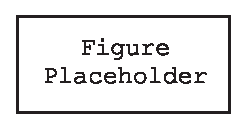
\includegraphics[width=4.6in]{c_cil0/lddvblk.eps}
\caption{Long Dividend Division Machine Instruction As A Functional Block}
\label{fig:ccil0:sidv0:sldm0:00}
\end{figure}

\begin{figure}
\centering
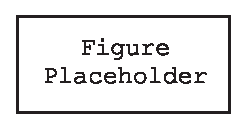
\includegraphics[width=4.6in]{c_cil0/ldmnblk.eps}
\caption{Long Dividend/Machine-Native Divisor Division In Functional Block Form}
\label{fig:ccil0:sidv0:sldm0:01}
\end{figure}

The following example illustrates how to apply the technique.

\begin{vworkexamplestatement}
\label{ex:ccil0:sidv0:sldm0:01}
Implement 32/8 unsigned division on the TMS370C8 processor, which is
characterized by a 16/8 division instruction.
\end{vworkexamplestatement}
\begin{vworkexampleparsection}{Solution}
It would be possible to prepare an implementation directly from
Figure \ref{fig:ccil0:sidv0:sldm0:01}:  however, it may be 
more instructive to work through a solution without the
aid of this figure.

In the case of the TMS370C8, the chunk size $Q$ is 8 bits; therefore
$Q=8$.  The problem statement indicates that we must accept 32-bit dividends;
therefore $P=32$.  Thus

\begin{equation}
\label{eq:ex:ccil0:sidv0:sldm0:01:001}
p = 2^{24} p_{[3]} + 2^{16} p_{[2]} + 2^{8} p_{[1]} + p_{[0]}
\end{equation}

\noindent{}and

\begin{equation}
\label{eq:ex:ccil0:sidv0:sldm0:01:002}
q = q_{[0]} .
\end{equation}

\noindent{}Thus the quotient and remainder we would like to determine,
$\lfloor p/q \rfloor$ and $p \bmod q$, can be obtained by repeated
application of (\ref{eq:ccil0:sidv0:sldm0:002}) as shown
in Equations (\ref{eq:ex:ccil0:sidv0:sldm0:01:003}) 
through (\ref{eq:ex:ccil0:sidv0:sldm0:01:011}).

\begin{equation}
\label{eq:ex:ccil0:sidv0:sldm0:01:003}
\frac{p}{q} 
=
\frac{2^{24} p_{[3]} + 2^{16} p_{[2]} + 2^{8} p_{[1]} + p_{[0]}}{q_{[0]}}
\end{equation}

\begin{equation}
\label{eq:ex:ccil0:sidv0:sldm0:01:004}
\frac{p}{q} 
=
2^{24} \frac{p_{[3]}}{q_{[0]}}
+
2^{16} \frac{p_{[2]}}{q_{[0]}}
+
2^{8} \frac{p_{[1]}}{q_{[0]}}
+
\frac{p_{[0]}}{q_{[0]}}
\end{equation}

\begin{equation}
\label{eq:ex:ccil0:sidv0:sldm0:01:005}
\frac{p}{q} 
=
2^{24} \left\lfloor{\frac{p_{[3]}}{q_{[0]}}}\right\rfloor
+
2^{24} \frac{(p_{[3]} \bmod q_{[0]})}{q_{[0]}}
+
2^{16} \frac{p_{[2]}}{q_{[0]}}
+
2^{8} \frac{p_{[1]}}{q_{[0]}}
+
\frac{p_{[0]}}{q_{[0]}}
\end{equation}

\begin{equation}
\label{eq:ex:ccil0:sidv0:sldm0:01:006}
\frac{p}{q} 
=
2^{24} \left\lfloor{\frac{p_{[3]}}{q_{[0]}}}\right\rfloor
+
2^{16} \frac{2^8 (p_{[3]} \bmod q_{[0]}) + p_{[2]}}{q_{[0]}}
+
2^{8} \frac{p_{[1]}}{q_{[0]}}
+
\frac{p_{[0]}}{q_{[0]}}
\end{equation}

\begin{eqnarray}
\label{eq:ex:ccil0:sidv0:sldm0:01:007}
\frac{p}{q} & = & 2^{24} \left\lfloor{\frac{p_{[3]}}{q_{[0]}}}\right\rfloor
+
2^{16} \left\lfloor{\frac{2^8 (p_{[3]} \bmod q_{[0]}) + p_{[2]}}{q_{[0]}}}\right\rfloor \\
\nonumber & + &
2^{16} \frac{(2^8 (p_{[3]} \bmod q_{[0]}) + p_{[2]}) \bmod q_{[0]}}{q_{[0]}}
+
2^{8} \frac{p_{[1]}}{q_{[0]}}
+
\frac{p_{[0]}}{q_{[0]}}
\end{eqnarray}

\begin{eqnarray}
\label{eq:ex:ccil0:sidv0:sldm0:01:008}
\frac{p}{q} & = & 2^{24} \left\lfloor{\frac{p_{[3]}}{q_{[0]}}}\right\rfloor
+
2^{16} \left\lfloor{\frac{2^8 (p_{[3]} \bmod q_{[0]}) + p_{[2]}}{q_{[0]}}}\right\rfloor \\
\nonumber & + &
2^{8} \frac{2^8((2^8 (p_{[3]} \bmod q_{[0]}) + p_{[2]}) \bmod q_{[0]}) + p_{[1]}}{q_{[0]}}
+
\frac{p_{[0]}}{q_{[0]}}
\end{eqnarray}

\begin{eqnarray}
\nonumber\frac{p}{q} & = & 2^{24} \left\lfloor{\frac{p_{[3]}}{q_{[0]}}}\right\rfloor
+
2^{16} \left\lfloor{\frac{2^8 (p_{[3]} \bmod q_{[0]}) + p_{[2]}}{q_{[0]}}}\right\rfloor \\
\label{eq:ex:ccil0:sidv0:sldm0:01:009}
 & + &
2^{8} \left\lfloor{\frac{2^8((2^8 (p_{[3]} \bmod q_{[0]}) + p_{[2]}) \bmod q_{[0]}) + p_{[1]}}{q_{[0]}}}\right\rfloor \\
\nonumber & + &
2^{8} \frac{(2^8((2^8 (p_{[3]} \bmod q_{[0]}) + p_{[2]}) \bmod q_{[0]}) + p_{[1]}) \bmod q_{[0]}}{q_{[0]}} \\
\nonumber & + &
\frac{p_{[0]}}{q_{[0]}}
\end{eqnarray}

\begin{eqnarray}
\nonumber\frac{p}{q} & = & 2^{24} \left\lfloor{\frac{p_{[3]}}{q_{[0]}}}\right\rfloor
+
2^{16} \left\lfloor{\frac{2^8 (p_{[3]} \bmod q_{[0]}) + p_{[2]}}{q_{[0]}}}\right\rfloor \\
\label{eq:ex:ccil0:sidv0:sldm0:01:010}
 & + &
2^{8} \left\lfloor{\frac{2^8((2^8 (p_{[3]} \bmod q_{[0]}) + p_{[2]}) \bmod q_{[0]}) + p_{[1]}}{q_{[0]}}}\right\rfloor \\
\nonumber & + &
\frac{2^8((2^8((2^8 (p_{[3]} \bmod q_{[0]}) + p_{[2]}) \bmod q_{[0]}) + p_{[1]}) \bmod q_{[0]}) + p_{[0]}}{q_{[0]}}
\end{eqnarray}

\begin{eqnarray}
\nonumber & \displaystyle \frac{p}{q} =  2^{24} \left\lfloor{\frac{p_{[3]}}{q_{[0]}}}\right\rfloor
+
2^{16} \left\lfloor{\frac{2^8 (p_{[3]} \bmod q_{[0]}) + p_{[2]}}{q_{[0]}}}\right\rfloor & \\
\label{eq:ex:ccil0:sidv0:sldm0:01:011}
 & \displaystyle + 
2^{8} \left\lfloor{\frac{2^8((2^8 (p_{[3]} \bmod q_{[0]}) + p_{[2]}) \bmod q_{[0]}) + p_{[1]}}{q_{[0]}}}\right\rfloor & \\
\nonumber & \displaystyle + 
\left\lfloor{\frac{2^8((2^8((2^8 (p_{[3]} \bmod q_{[0]}) + p_{[2]}) \bmod q_{[0]}) + p_{[1]}) \bmod q_{[0]}) + p_{[0]}}{q_{[0]}}}\right\rfloor + & \\
\nonumber 
& \displaystyle \frac{(2^8((2^8((2^8 (p_{[3]} \bmod q_{[0]}) + p_{[2]}) \bmod q_{[0]}) + p_{[1]}) \bmod q_{[0]}) + p_{[0]}) \bmod q_{[0]}}{q_{[0]}}
&
\end{eqnarray}

Note several things about the implementation suggested by 
(\ref{eq:ex:ccil0:sidv0:sldm0:01:011}):

\begin{itemize}
\item No addition or multiplication is required to calculate terms such as
      $2^8 (p_{[3]} \bmod q_{[0]}) + p_{[2]}$.  The high-order byte of the
      large dividend can be stuffed with $p_{[3]} \bmod q_{[0]}$ and
      the low-order byte with $p_{[2]}$.
\item No addition or multiplication is required to calculate the 
      result $\lfloor p/q \rfloor$.
      Note in (\ref{eq:ex:ccil0:sidv0:sldm0:01:011}) that the results are
      conveniently grouped as bytes with multipliers of $2^{24}$, 
      $2^{16}$, $2^8$, and $2^0=1$.  The terms can simply be placed into
      the appropriate byte, as a way of multplication by the appropriate
      power of 2.  Note also that each term is guaranteed to be
      $\in \{0, 1, 2, \ldots{} , 255\}$, by the argument presented
      earlier for (\ref{eq:ccil0:sidv0:sldm0:004}).  Thus, the
      addition will result in no carries, and each result byte can simply
      be placed directly in the correct memory location---addition is
      not necessary.
\item Four machine division instructions are required, and the remainder
      is produced automatically by the fourth instruction.
\end{itemize}

An implemenation for the TMS370C8 is supplied as Figure
\ref{fig:ex:ccil0:sidv0:sldm0:01:01}.  A block diagram of the data
flow for this implementation is supplied as 
Figure \ref{fig:ex:ccil0:sidv0:sldm0:01:02}.
\end{vworkexampleparsection}
\vworkexamplefooter{}

\begin{figure}
\begin{verbatim}
;Assume that byte memory locations p3, p2, p1, and p0 contain the
;32-bit unsigned dividend, and byte q0 contains the 8-bit unsigned
;divisor.  Assume also that the result quotient will be placed
;in byte memory locations d3, d2, d1, and d0; and that the
;remainder will be placed in the byte memory location r0.  Further
;assume that all memory locations are in the register file (near).
        CLR A        ;High-order chunk of large divisor
                     ;must be 0.
        MOV p3, B    ;Load the low-order chunk of divisor.
        DIV q0, A    ;Perform the first division.
        MOV A,  d3   ;Quotient becomes this part of the
                     ;result.
        MOV B,  A    ;Remainder becomes high-order chunk of
                     ;next division.
        MOV p2, B    ;Next byte becomes low-order chunk.
        DIV q0, A    ;Do the second division.
        MOV A,  d2   ;Quotient becomes this part of the
                     ;result.
        MOV B,  A    ;Remainder becomes high-order chunk of
                     ;next division.
        MOV p1, B    ;Next byte becomes low-order chunk.
        DIV q0, A    ;Do the third division.
        MOV A,  d1   ;Quotient becomes this part of the
                     ;result.
        MOV B,  A    ;Remainder becomes high-order chunk of
                     ;next division.
        MOV p0, B    ;Next byte becomes low-order chunk.
        DIV q0, A    ;Do the fourth division.
        MOV A,  d0   ;Quotient becomes this part of the
                     ;result.
        MOV B,  r0   ;This is the remainder, which could be used
                     ;for rounding.
\end{verbatim}
\caption{TMS370C8 Code Snippet Illustrating Unsigned 32/8 
         Division Using Unsigned 16/8
         Machine Instructions (Example \ref{ex:ccil0:sidv0:sldm0:01})}
\label{fig:ex:ccil0:sidv0:sldm0:01:01}
\end{figure}

\begin{figure}
\centering
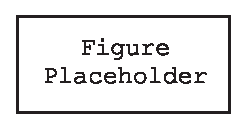
\includegraphics[width=4.6in]{c_cil0/t370dmp.eps}
\caption{Block Diagram Of Data Flow Of Figure \ref{fig:ex:ccil0:sidv0:sldm0:01:01}}
\label{fig:ex:ccil0:sidv0:sldm0:01:02}
\end{figure}


%%%%%%%%%%%%%%%%%%%%%%%%%%%%%%%%%%%%%%%%%%%%%%%%%%%%%%%%%%%%%%%%%%%%%%%%%%
%%%%%%%%%%%%%%%%%%%%%%%%%%%%%%%%%%%%%%%%%%%%%%%%%%%%%%%%%%%%%%%%%%%%%%%%%%
%%%%%%%%%%%%%%%%%%%%%%%%%%%%%%%%%%%%%%%%%%%%%%%%%%%%%%%%%%%%%%%%%%%%%%%%%%
\section{Miscellaneous Integer Mappings}
%Section tag: MIM0
\label{ccil0:smim0}

Embedded system work and ROM constraints often inspire a great deal
of cleverness in the selection of instructions to perform mappings or
tests.  In this section, we discuss integer mappings (i.e. functions)
for which economical implementations are known; and in the next section
(Section \ref{ccil0:smit0})
we discuss integer tests for which economical implementations are known.

To the best of our knowledge, there is no way to derive these mappings
and tests---they have been collected from many software developers and
come from human intuition and experience.


%%%%%%%%%%%%%%%%%%%%%%%%%%%%%%%%%%%%%%%%%%%%%%%%%%%%%%%%%%%%%%%%%%%%%%%%%%
%%%%%%%%%%%%%%%%%%%%%%%%%%%%%%%%%%%%%%%%%%%%%%%%%%%%%%%%%%%%%%%%%%%%%%%%%%
%%%%%%%%%%%%%%%%%%%%%%%%%%%%%%%%%%%%%%%%%%%%%%%%%%%%%%%%%%%%%%%%%%%%%%%%%%
\subsection{Lowest-Order Bit}
%Subsection tag: LIB0
\label{ccil0:smim0:slib0}

\index{lowest-order bit}
\index{least significant bit}

The mapping

\texttt{mask = x \& -x}

\noindent{}is the most economical way known to extract the 
lowest-order bit set in an integer \texttt{x}, or 
0 if no bits are set.\footnote{This mapping was contributed by 
David Baker (\texttt{bakerda@engin.umich.edu}) 
and Raul Selgado (\texttt{rselgado@visteon.com}).}  Since most processors have an instruction to form the
two's complement of an integer, this mapping usually requires only
two arithmetic instructions.

When implementing this mapping in assembly-language on processors without a
two's complement instruction, two other possible implementations are:

\begin{itemize}
\item \texttt{mask = x \& ($\sim$x + 1)}
\item \texttt{mask = x \& ((x \^{ } -1) + 1)}
\end{itemize}


%%%%%%%%%%%%%%%%%%%%%%%%%%%%%%%%%%%%%%%%%%%%%%%%%%%%%%%%%%%%%%%%%%%%%%%%%%
%%%%%%%%%%%%%%%%%%%%%%%%%%%%%%%%%%%%%%%%%%%%%%%%%%%%%%%%%%%%%%%%%%%%%%%%%%
%%%%%%%%%%%%%%%%%%%%%%%%%%%%%%%%%%%%%%%%%%%%%%%%%%%%%%%%%%%%%%%%%%%%%%%%%%
\section{Miscellaneous Integer Tests}
%Section tag: MIT0
\label{ccil0:smit0}

\subsection{Power Of 2}
%Subsection tag: PTW0
\label{ccil0:smit0:sptw0}

\index{power of two}
\index{2N@$2^N$}

The test

\texttt{(x \& (x-1) == 0) \&\& (x != 0)}

\noindent{}is the most economical way known to 
test whether an integer is a positive power of two 
(1, 2, 4, 8, 16, etc.).\footnote{The test appeared as part of
a discussion on 
the GMP mailing list in 2002.}


%%%%%%%%%%%%%%%%%%%%%%%%%%%%%%%%%%%%%%%%%%%%%%%%%%%%%%%%%%%%%%%%%%%%%%%%%%
%%%%%%%%%%%%%%%%%%%%%%%%%%%%%%%%%%%%%%%%%%%%%%%%%%%%%%%%%%%%%%%%%%%%%%%%%%
%%%%%%%%%%%%%%%%%%%%%%%%%%%%%%%%%%%%%%%%%%%%%%%%%%%%%%%%%%%%%%%%%%%%%%%%%%
\section{Exercises}

\begin{vworkexercisestatement}
\label{exe:ccil0:sexe0:01}
Show that any $m$-bit two's complement integer $u_{[m-1:0]}$ except
$-2^{m-1}$ can be negated by forming the one's complement, then adding one.
\end{vworkexercisestatement}



%%%%%%%%%%%%%%%%%%%%%%%%%%%%%%%%%%%%%%%%%%%%%%%%%%%%%%%%%%%%%%%%%%%%%%%%%%
%%%%%%%%%%%%%%%%%%%%%%%%%%%%%%%%%%%%%%%%%%%%%%%%%%%%%%%%%%%%%%%%%%%%%%%%%%
%%%%%%%%%%%%%%%%%%%%%%%%%%%%%%%%%%%%%%%%%%%%%%%%%%%%%%%%%%%%%%%%%%%%%%%%%%
\vfill
\noindent\begin{figure}[!b]
\noindent\rule[-0.25in]{\textwidth}{1pt}
\begin{tiny}
\begin{verbatim}
$HeadURL: svn://localhost/dtapublic/pubs/books/ucbka/trunk/c_cil0/c_cil0.tex $
$Revision: 277 $
$Date: 2019-08-12 22:35:39 -0400 (Mon, 12 Aug 2019) $
$Author: dashley $
\end{verbatim}
\end{tiny}
\noindent\rule[0.25in]{\textwidth}{1pt}
\end{figure}

%%%%%%%%%%%%%%%%%%%%%%%%%%%%%%%%%%%%%%%%%%%%%%%%%%%%%%%%%%%%%%%%%%%%%%%%%%
%
%End of file C_CIL0.TEX
